% epaData — CS396 Phase 2 project report.
% Build from the repository root: npm run report  (writes report/phase2/phase2-report.pdf)
\documentclass[11pt,a4paper]{article}

% Shared preamble of the epaData reports (main.tex: Phase 1, phase2.tex: Phase 2).

\usepackage[margin=2.5cm]{geometry}
\usepackage{fontspec}
\usepackage{microtype}
\usepackage{amsmath,amssymb}
\usepackage{graphicx}
\usepackage{booktabs}
\usepackage{tabularx}
\usepackage{longtable}
\usepackage{array}
\usepackage{xcolor}
\usepackage{listings}
\usepackage{caption}
\usepackage{float}
\usepackage{enumitem}
\usepackage{tikz}
\usetikzlibrary{positioning,arrows.meta,shapes.multipart,fit,calc,backgrounds}
\usepackage[hidelinks]{hyperref}
\usepackage{url}
\usepackage[htt]{hyphenat}
\setlength{\emergencystretch}{2.5em}

\graphicspath{{figures/}}
\setlength{\parskip}{0.45em}
\setlength{\parindent}{0pt}
\captionsetup{font=small,labelfont=bf}
\setlist{itemsep=0.15em,topsep=0.3em}

% Chemistry and units used throughout the text.
\newcommand{\COtwo}{CO\textsubscript{2}}
\newcommand{\SOtwo}{SO\textsubscript{2}}
\newcommand{\NOx}{NO\textsubscript{x}}
\newcommand{\code}[1]{\texttt{#1}}
\newcolumntype{L}{>{\raggedright\arraybackslash}X}
\newcolumntype{R}[1]{>{\raggedright\arraybackslash}p{#1}}

% ---------------------------------------------------------------- listings
\definecolor{codebg}{RGB}{248,248,246}
\definecolor{codekw}{RGB}{0,92,158}
\definecolor{codestr}{RGB}{163,21,21}
\definecolor{codecom}{RGB}{96,120,96}
\lstset{
  basicstyle=\ttfamily\footnotesize,
  backgroundcolor=\color{codebg},
  keywordstyle=\color{codekw}\bfseries,
  stringstyle=\color{codestr},
  commentstyle=\color{codecom}\itshape,
  numbers=left, numberstyle=\tiny\color{gray}, numbersep=6pt,
  frame=single, rulecolor=\color{black!15}, framesep=4pt,
  breaklines=true, columns=fullflexible, keepspaces=true,
  showstringspaces=false, tabsize=2, captionpos=b,
  xleftmargin=1.4em, framexleftmargin=1.4em,
}
\lstdefinelanguage{TypeScript}{
  keywords={const,let,function,async,await,return,if,else,for,of,in,new,export,import,from,type,interface,true,false,undefined,null,typeof},
  sensitive=true, morecomment=[l]{//}, morecomment=[s]{/*}{*/},
  morestring=[b]", morestring=[b]', morestring=[b]`,
}
\lstdefinestyle{sql}{language=SQL, morekeywords={OVER,PARTITION,ROW_NUMBER,LIMIT,OFFSET,EXISTS,COALESCE,NULLIF,IF,REFERENCES,CASCADE,UNIQUE,INDEX}}

% ---------------------------------------------------------------- TikZ styles
\tikzset{
  box/.style={draw, rounded corners=2pt, align=center, font=\small, inner sep=5pt, fill=white},
  store/.style={box, fill=black!4},
  ext/.style={box, dashed},
  flow/.style={-{Latex[length=2mm]}, thick},
  lflow/.style={-{Latex[length=2mm]}, thick, dashed},
  lbl/.style={font=\scriptsize, fill=white, inner sep=1.5pt},
}


\newcommand{\PMtwofive}{PM\textsubscript{2.5}}

\title{%
  \vspace*{-1em}
  {\Large CS396 Project Phase 2 Report}\\[0.8em]
  \textbf{epaData}: Analysis, Impact Assessment, and Prediction\\for EPA Power-Sector Emissions Data}
\author{Raaj Banga \and Arnav Bawankule}
\date{November 2026}

\begin{document}
\maketitle

\begin{abstract}
\noindent
Phase~1 of epaData built a database of the annual operating and emissions data that U.S.\
power-plant units report to the EPA Clean Air Markets Program (CAMPD), with retrieval, upload,
validation, search, and export. Phase~2 turns that database into a decision-support tool. An
\emph{Analyze} page lets a user select unit-years with the Phase~1 filters and then summarize
them with descriptive statistics, derive normalized indicators such as emission intensities,
heat rate, capacity factor, and year-over-year change, explore them in interactive charts,
compare groups with confidence intervals and hypothesis tests, and convert \COtwo{}, \SOtwo{},
and \NOx{} emissions into EPA TRACI~2.2 potential-impact indicators. A \emph{Predict} page
compares a baseline with Ridge regression and a decision tree that predict a unit's annual
\NOx{} emissions; on the held-out reporting years 2024--2025 the tree reaches $R^2 = 0.951$
against $0.489$ for the baseline. The same models drive one-variable sensitivity curves and
named what-if scenarios, with warnings when an input leaves the training data. Every result can
be exported with metadata that records how it was produced. This report documents the
analytical questions, the methods and their assumptions, the design, the results, and the
limitations of the system.
\end{abstract}

\tableofcontents
\newpage

% ------------------------------------------------------------------------
\section{Project description}
\label{sec:description}

\subsection{Problem}

Phase~1 made CAMPD data easy to find and trust: a user can ask which Kentucky coal units emitted
more than 500{,}000 tons of \COtwo{} in 2025 and see where every number came from. It could not
answer the questions that follow. Is the sector's \COtwo{} falling because plants are getting
cleaner or because generation is moving between fuels? Do units with selective catalytic
reduction (SCR) really emit less \NOx{} per unit of fuel, and by how much? Which states
contribute most to acidification, and does the ranking change once the result is divided by
the electricity produced? How much \NOx{} would a particular unit emit if it burned 5\,\% less
fuel or added a control?

Answering such questions requires statistics over many unit-years with a correct treatment of
missing values, indicators that are comparable across plants of different size, a defensible
link between emitted mass and environmental impact, and a model whose predictions are evaluated
honestly before they are used for what-if analysis.

\subsection{Analytical questions}

Phase~2 is organized around four questions, each answered with a function of the application
(Section~\ref{sec:results}):
\begin{enumerate}[label=Q\arabic*.]
  \item How have emissions and emission intensity changed between 2015 and 2025, and how much of
        the change is a shift from coal to gas?
  \item How large is the difference in \NOx{} emission rate between units with and without
        post-combustion \NOx{} control, and is it statistically distinguishable from chance?
  \item Which states and facilities contribute most to each TRACI impact category, in total and
        per MWh?
  \item How well can a unit's annual \NOx{} emissions be predicted from its operating data,
        attributes, controls, and history, and how do predictions respond to changed inputs?
\end{enumerate}

\subsection{Intended users}

The specification names environmental researchers, power-sector analysts, regulators, facility
managers, students, and the interested public. Phase~2 assumes these users know their domain
but not statistics software: every statistic is labeled with its unit and definition, every
test is accompanied by a plain-language reading, and every model result is labeled as a model
response rather than a measured effect.

\subsection{Objectives}

Phase~2 addresses the course objectives deferred from Phase~1, O8 (environmental indicators),
O9 (multi-criteria evaluation), and O10 (interactive charts of evaluation results), through the
nine goals of the Phase~2 specification: explore the data with descriptive statistics; compare
facilities, units, fuels, states, and periods; visualize emissions and operating data; estimate
potential impacts with TRACI factors; identify trends, relationships, and unusual observations;
build and evaluate prediction models; perform sensitivity and scenario analysis; save and export
results; and explain methods, assumptions, results, and limitations. Section~\ref{sec:testing}
assesses each goal.

\subsection{Scope}

Phase~2 uses the CAMPD records of the Phase~1 database and the TRACI~2.2 characterization
factors for the three pollutants CAMPD reports (\COtwo{}, \SOtwo{}, and \NOx{} emitted to air).
Analyses default to the complete reporting years 2015--2025 retrieved from the CAMPD API; the
older uploaded years (1996--1998 and 2006--2008) and the partial year 2026 remain selectable but
are excluded from model training. The prediction target is annual \NOx{} mass per unit-year
(Section~\ref{sec:prediction}). Multi-criteria weighted scoring, listed among the course
objectives, is not part of the Phase~2 specification and was not built.

% ------------------------------------------------------------------------
\section{Functions implemented}
\label{sec:functions}

Two pages were added between \emph{Map} and \emph{Retrieve} in the navigation bar:
\emph{Analyze} (\code{/analyze}), with the tabs Dataset, Statistics, Charts, Compare, and
Impacts, and \emph{Predict} (\code{/predict}), with the tabs Models, Sensitivity, and Scenarios.
As in Phase~1, the URL holds the complete state of a page (filters, tab, and every choice on the
tab), so any view can be reloaded, bookmarked, or shared.

\subsection{Analytical dataset builder}

The Analyze page reuses the Explore page's filter bar without change: reporting-year range,
state, facility, unit, primary and secondary fuel, unit type, \SOtwo{}, \NOx{}, and particulate
controls, program, operating status, record origin, audit flags, and minimum and maximum
operating time, gross load, heat input, and emitted mass. The selected unit-years are the
analytical dataset for every tab. The Dataset tab (Figure~\ref{fig:dataset}) reports how many
unit-years, facilities, units, and years were selected, lists every variable with its kind,
unit, definition, how groups combine it, and how many of its values are missing, and lists the
fields the selection can be grouped by with their number of distinct values. A \emph{Download
dataset} button exports every selected unit-year with all variables
(Section~\ref{sec:exports}).

\begin{figure}[H]
  \centering
  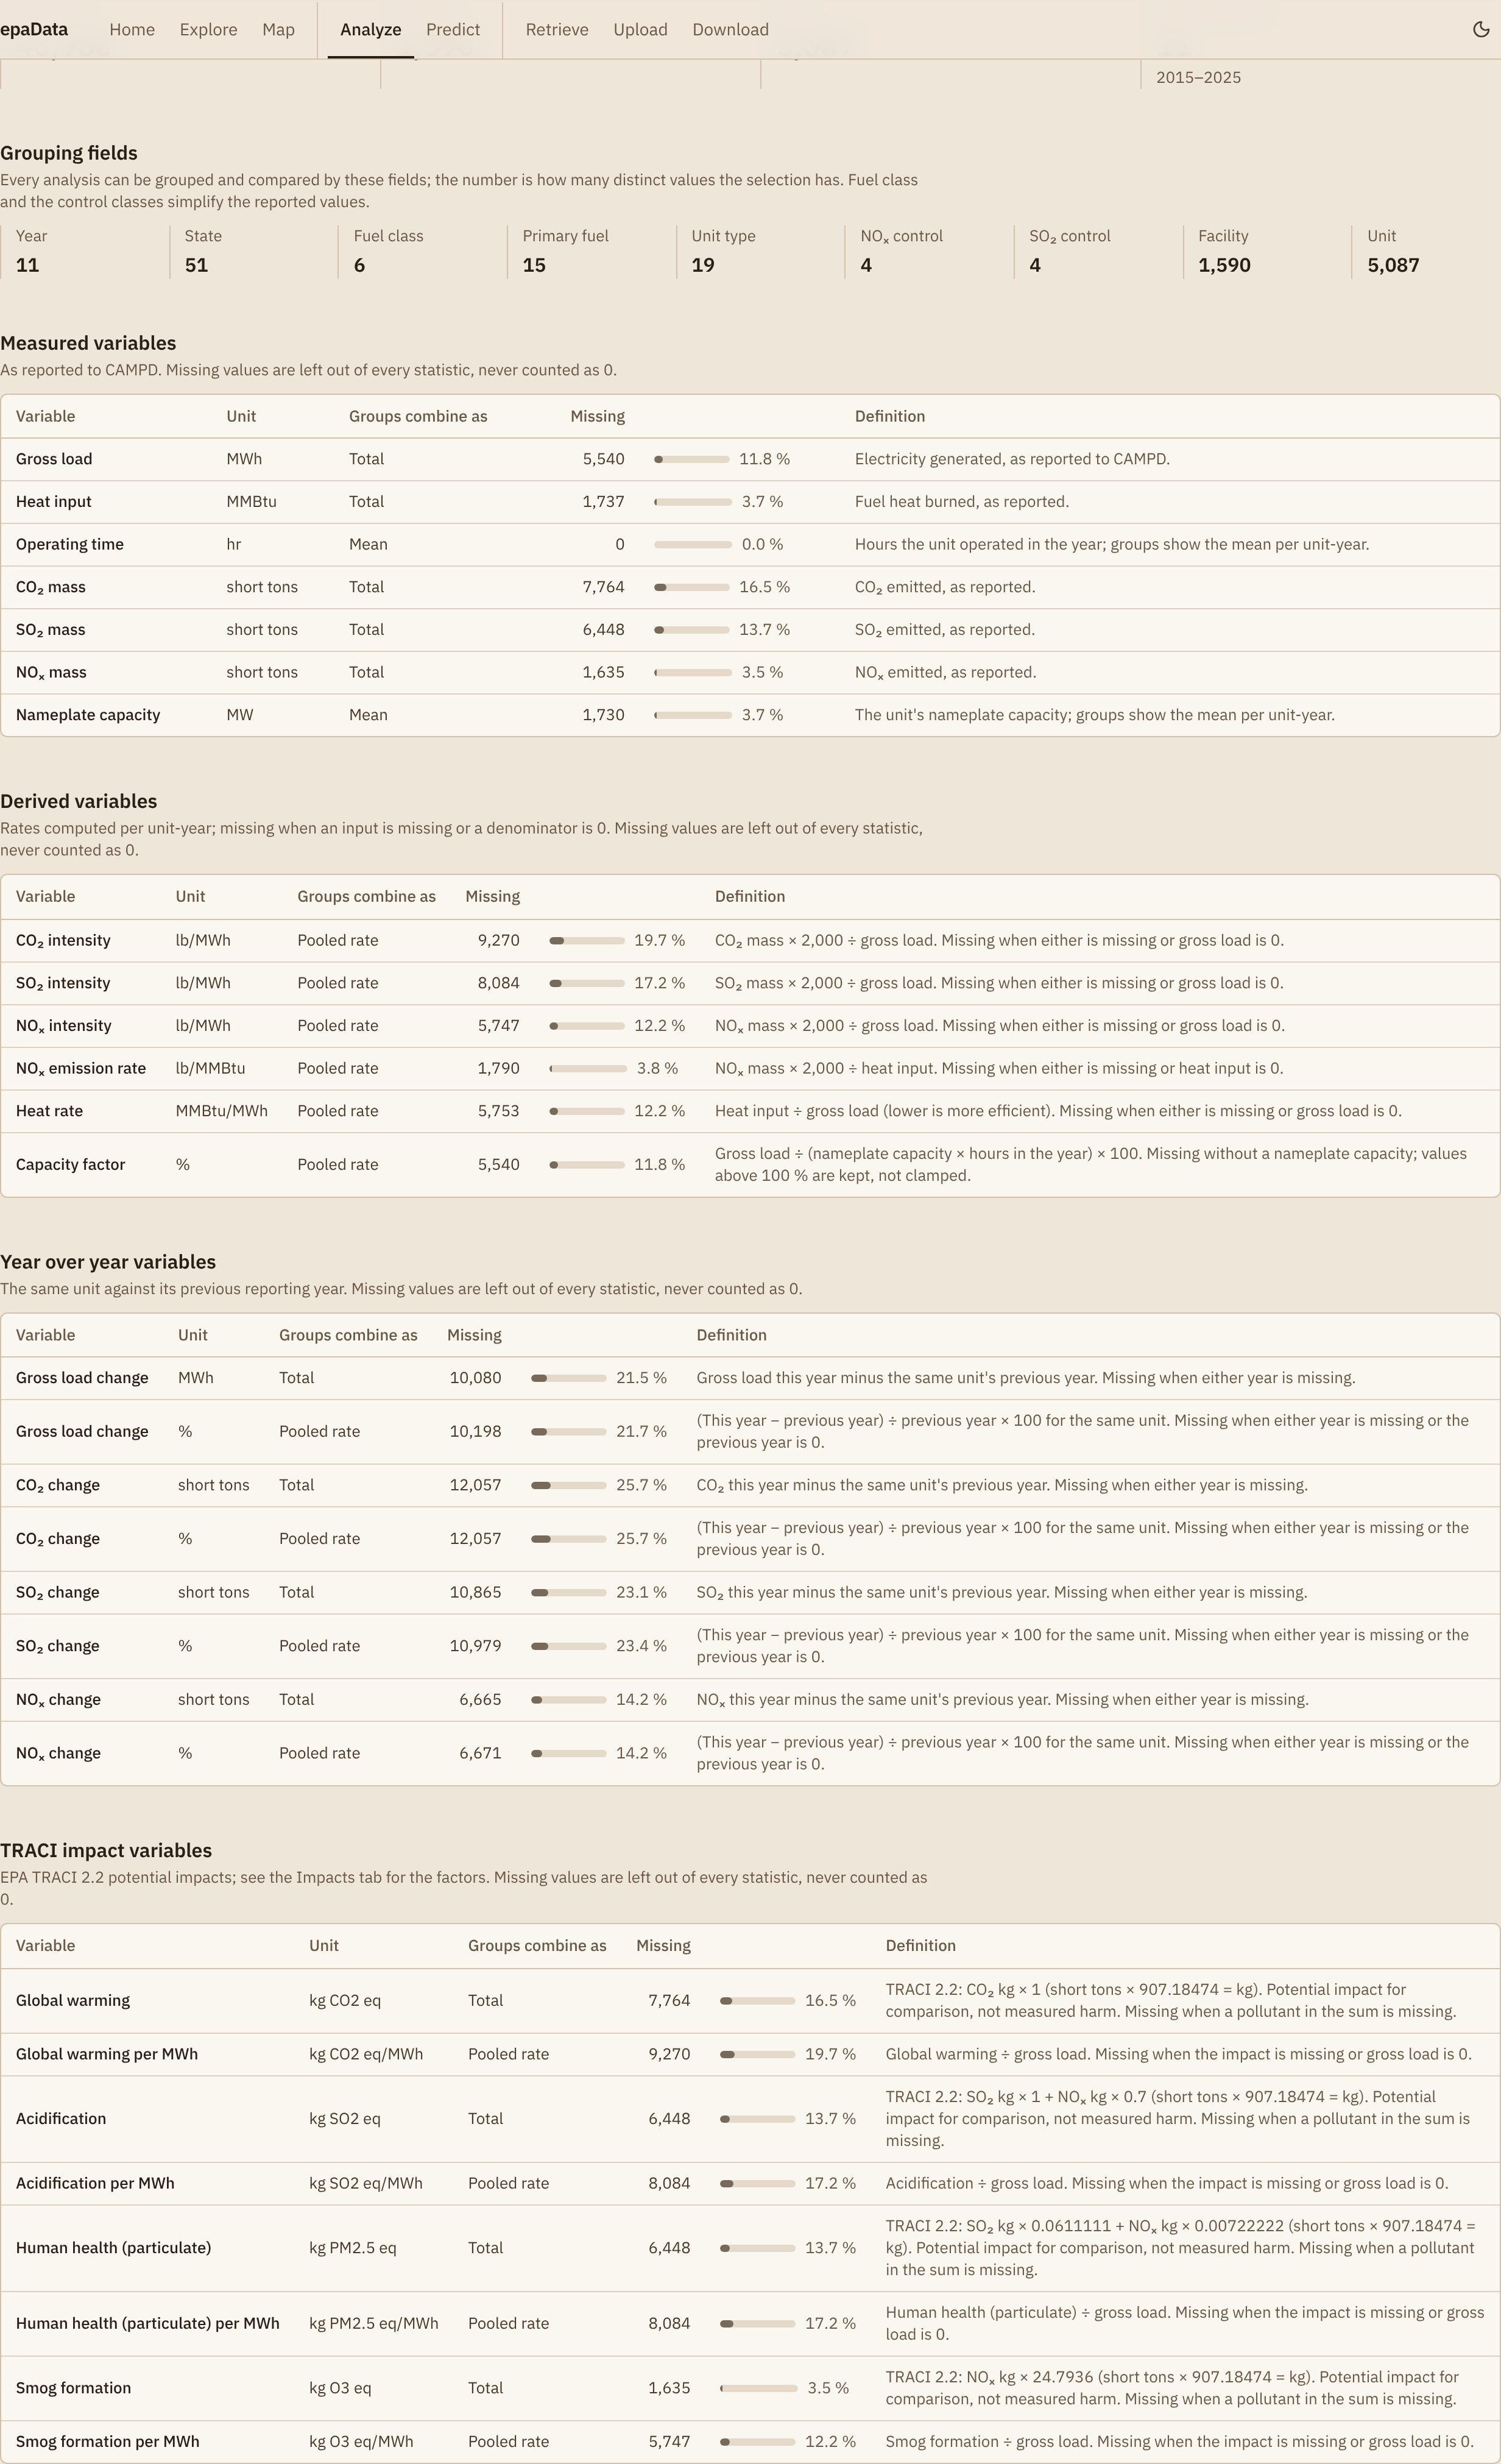
\includegraphics[width=\linewidth]{p2-dataset.jpg}
  \caption{Dataset tab for 2015--2025: 46{,}988 unit-years of 1{,}590 facilities and 5{,}087
  units. Each variable is listed with its kind, unit, how groups combine it, and its missing
  values.}
  \label{fig:dataset}
\end{figure}

\subsection{Derived indicators}

Twenty-nine variables are available (Table~\ref{tab:variables}): seven measured values, six
derived rates, eight year-over-year changes, and eight TRACI indicators. The derived and TRACI
variables are computed from the stored records whenever an analysis runs, so they always agree
with the current data. Section~\ref{sec:methods} gives their definitions and the rules for
missing values.

\subsection{Descriptive statistics}

The Statistics tab (Figure~\ref{fig:statistics}) describes one variable over the selection:
count, missing count, minimum, maximum, mean, median, standard deviation, first and third
quartiles, interquartile range, and the 5th, 10th, 90th, and 95th percentiles, together with the
variable's total, mean, or pooled rate over the whole selection. With a grouping field it
repeats these statistics for each group in a sortable table. It also lists \emph{unusual
observations}: the unit-years beyond Tukey's far-out fences, $Q_1 - 3\,\text{IQR}$ and
$Q_3 + 3\,\text{IQR}$, with their count on each side and the ten most extreme. The four example questions of the
specification (average \COtwo{} by state, median \NOx{} intensity by fuel, total \SOtwo{} by
year, and average heat rate by unit type) are offered as one-click examples.

\begin{figure}[H]
  \centering
  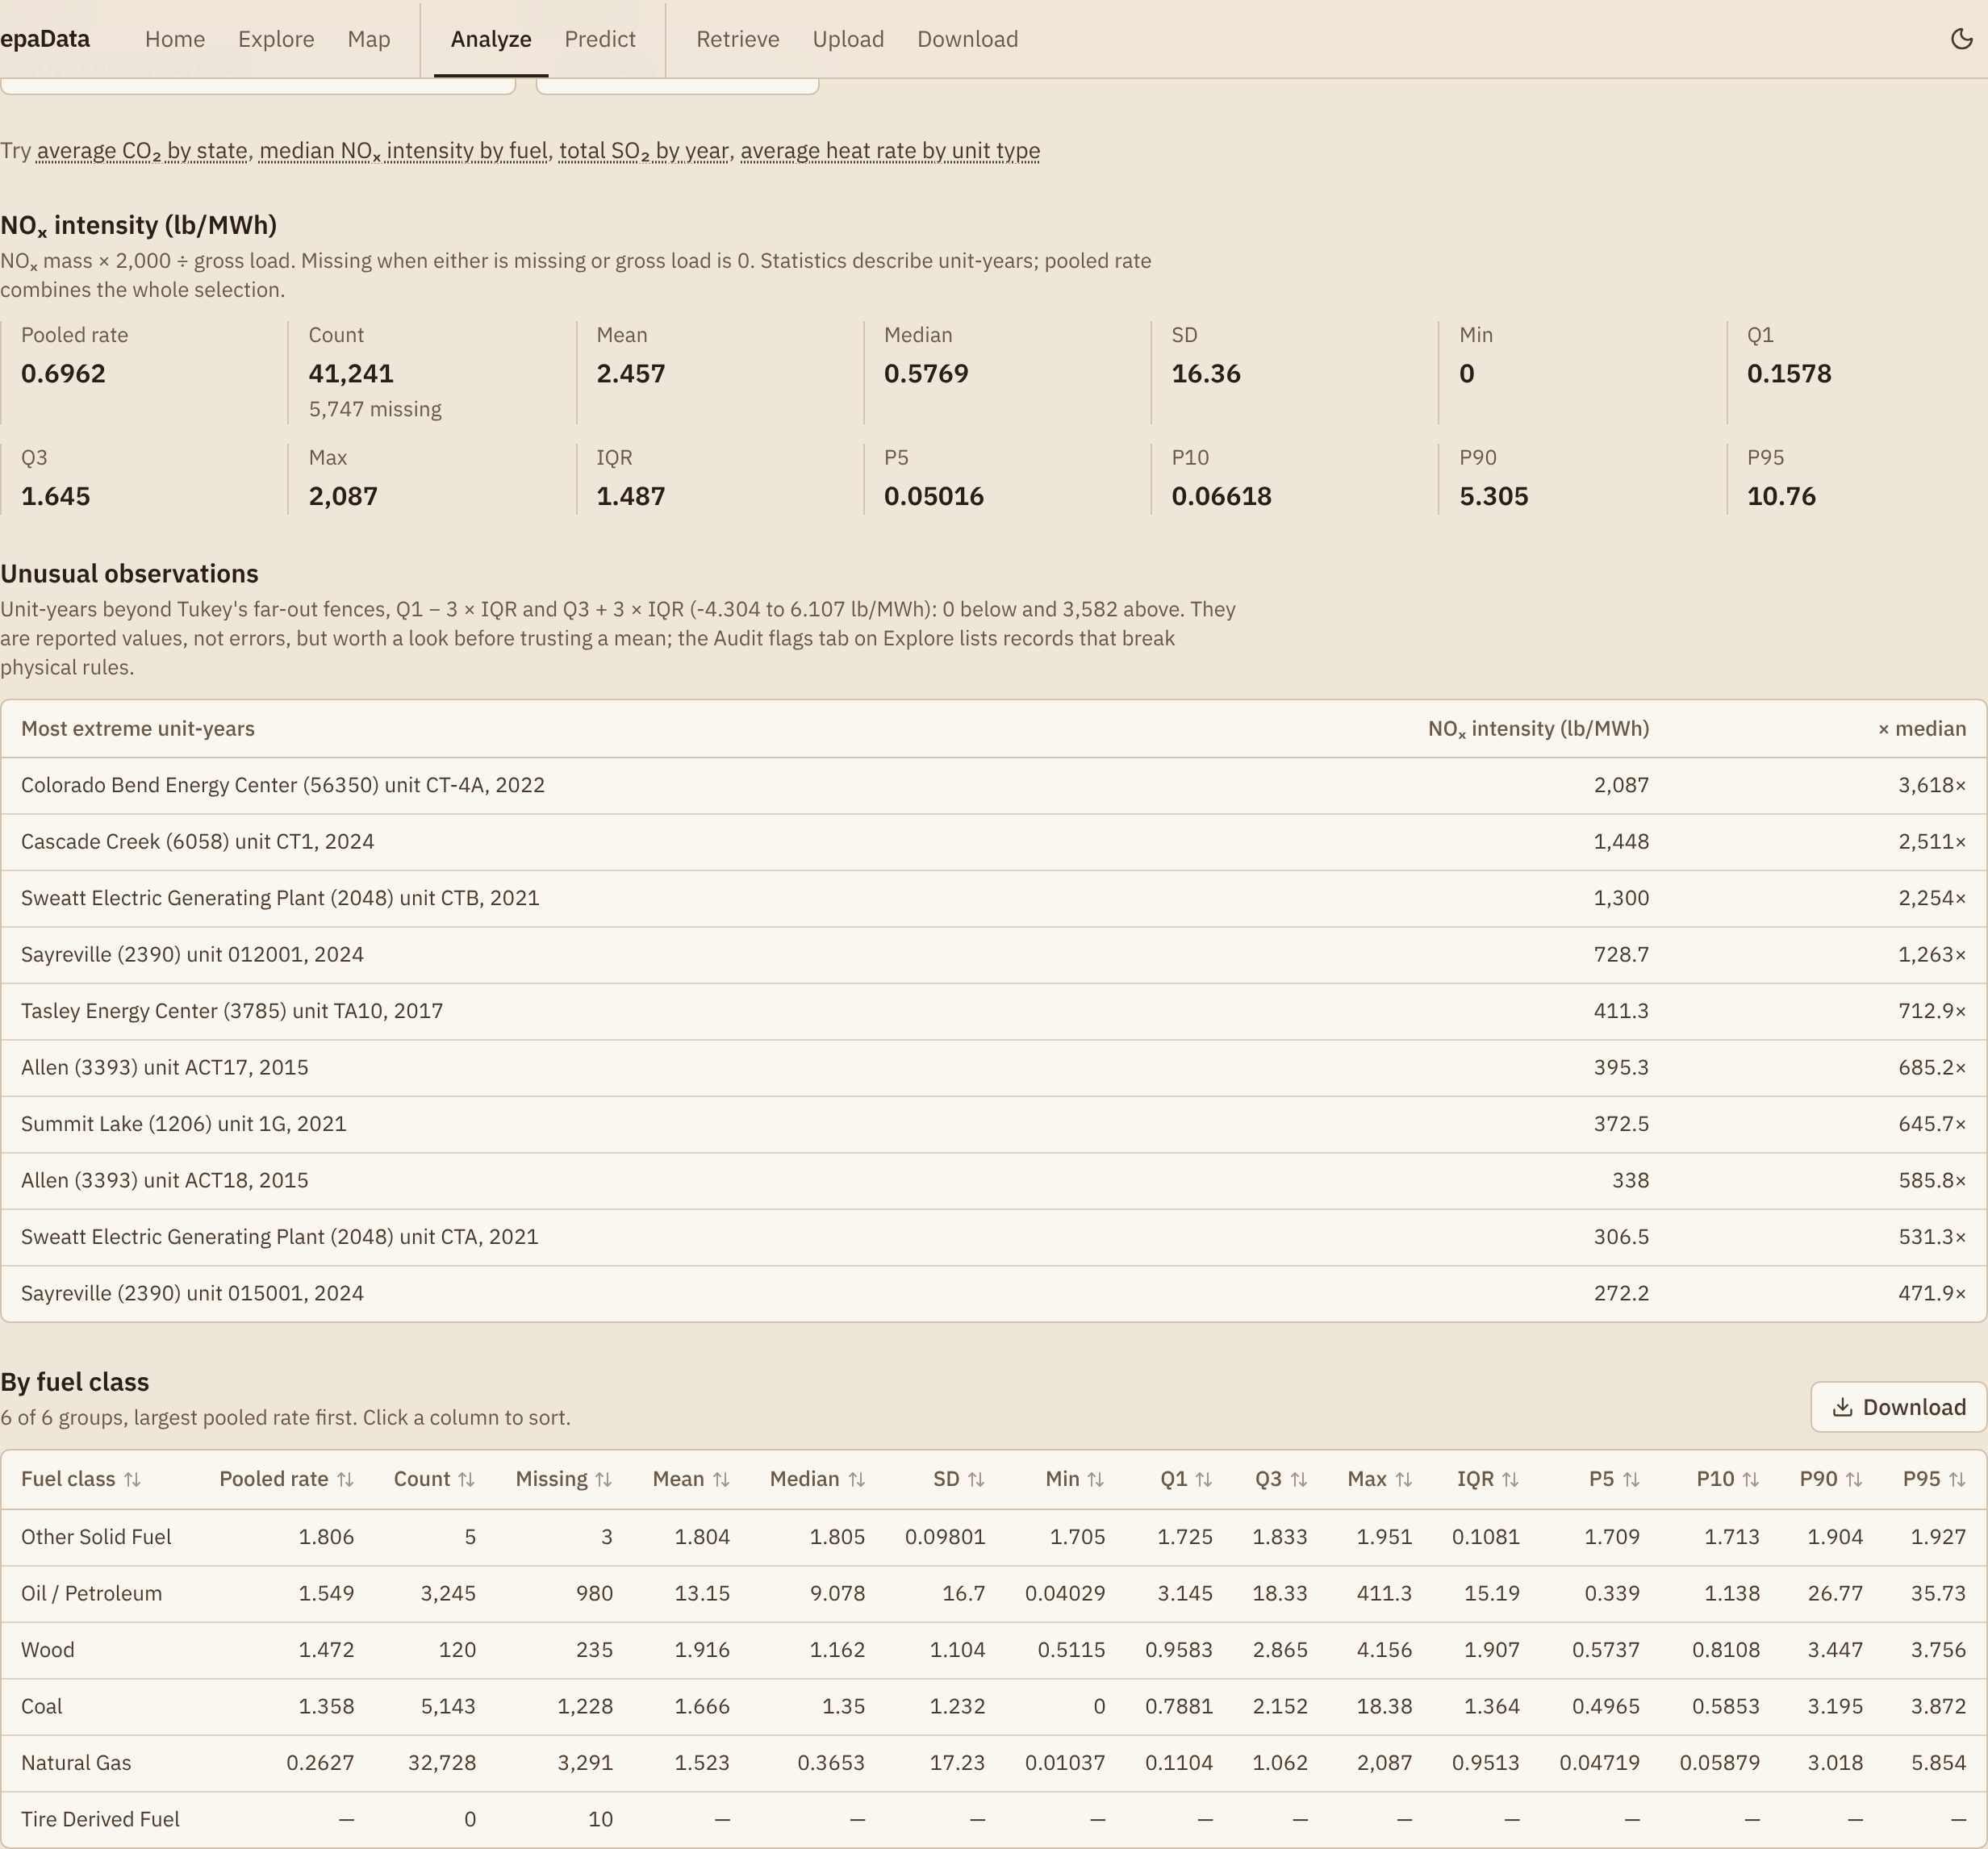
\includegraphics[width=\linewidth]{p2-statistics.jpg}
  \caption{Statistics tab: \NOx{} intensity over 2015--2025, overall and by fuel class.}
  \label{fig:statistics}
\end{figure}

\subsection{Interactive visualization}

The Charts tab draws seven chart types with Plotly.js~\cite{plotly}, all over the same selection:
a trend of any variable per year with one line per group; bars per group; histograms and box
plots, optionally on a logarithmic scale and split by group; scatter plots of any two variables
colored by group; a Pearson or Spearman correlation heat map of eleven variables; the highest or
lowest twenty facilities or units; and a state choropleth. Every chart has a descriptive title,
axis titles with units, a legend, tooltips with values and counts, zoom, PNG export, and a
\emph{Data} button that saves its data, image, and metadata. Fuel classes keep the colors they
have on the Phase~1 map. Distributions and scatter plots of very large selections are drawn
from an even sample of 20{,}000 values or 4{,}000 points, which the chart states; correlations
and statistics always use every value.

\subsection{Comparative analysis}

The Compare tab compares two to eight groups along any grouping field: states, fuels, unit
types, \NOx{} or \SOtwo{} control classes (for example units with and without SCR), or
reporting years (for example 2015 against 2024). For each group it shows the pooled value of the
variable, its rank among the compared groups, its difference and percentage difference from the
first group, the count, the mean
with its 95\,\% confidence interval, the median, and the standard deviation; it runs Welch's
$t$-test and the Mann--Whitney $U$ test for two groups and one-way ANOVA and the
Kruskal--Wallis test for any number; and it states the result in plain language with its caveats
(Figure~\ref{fig:compare}). The Phase~1 comparison of two to four individual facilities or
units remains available from the Explore page.

\subsection{Environmental and health impact indicators}

The Impacts tab converts the selected emissions into four TRACI~2.2 impact categories, global
warming, acidification, particulate-matter human health, and smog formation, grouped by any
field. Each category is shown in its own equivalent unit, both as a total and per MWh of gross
load, and is never added to another category. The tab shows the factors used, with their TRACI
version, substance, CAS number, and unit, and the formula of each category, and it states that
the results are potential impacts for comparison, not measured harm (Figure~\ref{fig:impacts}).

\subsection{Prediction}

The Models tab of the Predict page compares the three registered models, a baseline, Ridge
regression, and a decision tree, on the validation and test years; plots predicted against
actual \NOx{} for the test years; shows the tree's feature importances or the Ridge
coefficients; and records each model's inputs, split, saved file, software versions, and
training time (Figure~\ref{fig:models}).

\subsection{Sensitivity and scenario analysis}

The Sensitivity and Scenarios tabs start from a baseline unit-year, chosen by facility name or
ID, year, and unit, and a model. Sensitivity varies one input from a minimum to a maximum value, entered
either in the input's own unit or as percentages of its baseline value, with all other inputs
held constant, and draws the prediction as a curve with the
baseline marked and the region outside the training data shaded (Figure~\ref{fig:sensitivity}).
Scenarios compares the baseline with five named changes, gross load $+10\,\%$, heat input
$-5\,\%$ (both editable), adding or removing SCR, switching the primary fuel, and a combined
high-efficiency case, for both trained models side by side (Figure~\ref{fig:scenarios}).

\subsection{Saving and exporting results}
\label{sec:exports}

Every chart's \emph{Data} button and every statistics and impact table downloads a ZIP file
containing the data as CSV, the chart as PNG when there is one, and a \code{metadata.json} file.
The metadata records the export time and URL; the software version and Git commit; a snapshot of
the database (unit-years, datasets, and last import); the filters and every tab choice; the
definition, unit, and aggregation of each variable shown; the TRACI factors for impact results;
and, on the Predict page, the model's inputs, settings, split years, metrics, saved file, and
software versions, and the baseline unit-year. The complete analytical dataset is exported by
the server (\code{/api/export?type=analysis}) in the same format.

\subsection{Requirement traceability}

Table~\ref{tab:trace} maps each requirement of the Phase~2 specification to the function that
meets it.

{\small
\begin{longtable}{@{}R{0.26\linewidth}R{0.55\linewidth}R{0.12\linewidth}@{}}
\caption{Phase~2 requirements and where they are met.}\label{tab:trace}\\
\toprule
\textbf{Specification} & \textbf{epaData} & \textbf{Status}\\
\midrule\endfirsthead
\toprule
\textbf{Specification} & \textbf{epaData} & \textbf{Status}\\
\midrule\endhead
\S3 CAMPD multi-year data & 2015--2025 API years (and older uploads) in \code{annual\_records} & Met\\
\S3 TRACI version, pollutant, category, factor, unit stored & \code{traci\_factors} table & Met\\
\S4.1 Dataset builder: years, state, facility, unit, fuel, unit type, controls, program, minimum operating time or load & Explore filter bar on Analyze & Met\\
\S4.1 Record, facility, unit, year counts; missing-value summary; variables & Dataset tab & Met\\
\S4.1 Reproducible through URL or saved configuration & URL parameters; exported metadata & Met (URL)\\
\S4.2 Count, missing, min, max, mean, median, SD, quartiles, IQR, percentiles; grouped & Statistics tab & Met\\
\S4.3 \COtwo{}, \SOtwo{}, \NOx{} intensity; heat rate; year-over-year change; utilization & Derived variables; capacity factor & Met\\
\S4.3 Division by zero and missing values stay missing & Variable rules; tests & Met\\
\S4.4 Line, bar, histogram, box, scatter, correlation heat map, rankings, state map & Charts tab & Met\\
\S4.4 Titles, units, legends, tooltips, filters, image and data download & \code{Chart} component & Met\\
\S4.5 Facilities, units, states, fuels, unit types, with and without control, periods & Compare tab; Phase~1 compare dialog & Met\\
\S4.5 Statistics, differences, rankings, charts, normalized indicators; tests; plain language & Compare tab & Met\\
\S4.6 Short tons to kg; exact pollutant matching; sum within category; per MWh; record factors & Impacts tab; \code{impactVariables} & Met\\
\S5.1 One prediction target & Annual \NOx{} mass per unit-year & Met\\
\S5.2 Features; no target leakage & Section~\ref{sec:prediction}; ablation & Met\\
\S5.3 Baseline and at least two models & Median baseline, Ridge, decision tree & Met\\
\S5.4 Chronological split; MAE, RMSE, $R^2$, MAPE & 2016--21 / 2022--23 / 2024--25 & Met\\
\S6.2 One variable at a time & Sensitivity tab & Met\\
\S6.3 Scenarios with range warnings & Scenarios tab & Met\\
\S6.4 Curve, baseline marks, scenario bars, tooltips, out-of-range shading & Sensitivity and Scenarios tabs & Met\\
\S7 Export datasets, statistics, models, sensitivity, scenarios, charts, with metadata & ZIP exports & Met\\
\S8.1 Flask, Jinja2, SQLAlchemy, pandas, scikit-learn, joblib, pytest & Next.js, React, Drizzle; pandas, scikit-learn, joblib, pytest offline (Section~\ref{sec:design}) & Changed\\
\S12.3 Instructions, migrations, tests, fixtures, no keys & README, migration 0009, 57 + 6 tests & Met\\
\bottomrule
\end{longtable}}

\subsection{Planned functions not completed or changed}

Table~\ref{tab:changes} compares the Phase~2 plan with the delivered system.

{\small
\begin{longtable}{@{}R{0.26\linewidth}R{0.27\linewidth}R{0.41\linewidth}@{}}
\caption{Plan versus delivered system.}\label{tab:changes}\\
\toprule
\textbf{Planned} & \textbf{Delivered} & \textbf{Reason}\\
\midrule\endfirsthead
\toprule
\textbf{Planned} & \textbf{Delivered} & \textbf{Reason}\\
\midrule\endhead
Store derived rates as columns & Computed when an analysis runs & Always consistent with the records; no backfill after imports.\\
Eutrophication from \NOx{} & Not provided & The TRACI~2.2 workbook has no eutrophication column.\\
Partial impact when a pollutant is missing & Category missing for that unit-year & A partial sum would understate the impact silently.\\
State and capacity factor as model inputs & Left out & State is sparse for many fuel and type combinations; capacity factor duplicates gross load and nameplate capacity.\\
Saved analysis configurations & URL parameters only & The URL already reproduces a view; saving it is a bookmark.\\
Gradient-boosting model for comparison & Not built & Time; the tree already reaches $R^2 = 0.95$.\\
\bottomrule
\end{longtable}}

% ------------------------------------------------------------------------
\section{System design}
\label{sec:design}

\subsection{Architecture}

Phase~2 keeps the Phase~1 stack: Next.js~16 with React~19 on the web layer, tRPC procedures for
typed calls from the browser, Drizzle ORM, and SQLite. The specification recommends Flask with
pandas and scikit-learn; the Phase~1 report explained the mapping of Flask, Jinja, and
SQLAlchemy to the stack used. For the analytical work we adopted a hybrid
(Figure~\ref{fig:architecture}). Statistics, indicators, and TRACI impacts are computed in
TypeScript on the server, close to the database. Models are trained offline in Python with
pandas and scikit-learn~\cite{pedregosa2011sklearn}, and each trained model is stored in the
database with its preprocessing and parameters as JSON, which a small TypeScript module replays
exactly. Predictions, sensitivity curves, and scenarios are therefore instant, need no Python
process at request time, and work on the read-only hosted build, where Python is unavailable.

\begin{figure}[H]
  \centering
  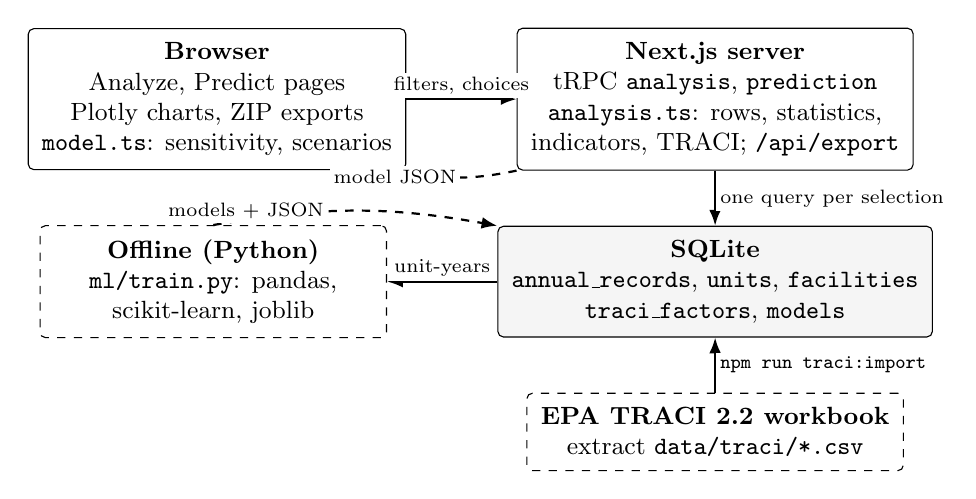
\begin{tikzpicture}[node distance=7mm and 9mm]
    \node[box, minimum width=4.4cm] (pages) {\textbf{Browser}\\Analyze, Predict pages\\Plotly charts, ZIP exports\\\code{model.ts}: sensitivity, scenarios};
    \node[box, right=14mm of pages, minimum width=4.6cm] (server) {\textbf{Next.js server}\\tRPC \code{analysis}, \code{prediction}\\\code{analysis.ts}: rows, statistics,\\indicators, TRACI; \code{/api/export}};
    \node[store, below=of server, minimum width=4.6cm] (db) {\textbf{SQLite}\\\code{annual\_records}, \code{units}, \code{facilities}\\\code{traci\_factors}, \code{models}};
    \node[ext, left=14mm of db, minimum width=4.4cm] (train) {\textbf{Offline (Python)}\\\code{ml/train.py}: pandas,\\scikit-learn, joblib};
    \node[ext, below=of db, minimum width=4.6cm] (traci) {\textbf{EPA TRACI 2.2 workbook}\\extract \code{data/traci/*.csv}};
    \draw[flow] (pages) -- node[lbl, above] {filters, choices} (server);
    \draw[flow] (server) -- node[lbl, right] {one query per selection} (db);
    \draw[flow] (db) -- node[lbl, above] {unit-years} (train);
    \draw[lflow] (train.north) to[bend left=10] node[lbl, left, pos=0.4] {models + JSON} (db.north west);
    \draw[flow] (traci) -- node[lbl, right] {\code{npm run traci:import}} (db);
    \draw[lflow] (server.south west) to[bend left=12] node[lbl, left, pos=0.5] {model JSON} (pages.south east);
  \end{tikzpicture}
  \caption{Phase~2 architecture. Solid arrows run on every request or import; dashed arrows
  carry the trained models from the offline pipeline to the browser.}
  \label{fig:architecture}
\end{figure}

\subsection{Life cycle of an analysis}

When a tab needs a result, the browser calls a tRPC procedure with the filters and the tab's
choices. The server turns the filters into the same SQL conditions the Explore page uses (one
shared function, \code{unitYearConditions}), and selects the matching unit-years joined with
their unit, facility, and the same unit's previous year, which the year-over-year variables need.
The rows are cached for 60~seconds, since one page typically asks for several views of the same
selection; the variables are then evaluated in memory and only the result (a table, a set of
chart points, a matrix) is returned. The complete 2015--2025 selection of 46{,}988 unit-years
loads in about 1.3~s on a laptop, and each subsequent view over it is computed in about
0.1~s.

\subsection{Database additions}

Migration 0009 adds two tables. \code{traci\_factors} holds one row per TRACI version,
pollutant, medium, and impact category, with the TRACI substance name and CAS number, the factor,
its unit, and the workbook column it was read from; a unique index prevents duplicates. It is
loaded from a six-row extract of the EPA workbook (\code{data/traci/traci\_2\_2\_air.csv}), whose
source, download date, and checksum are recorded beside it. \code{models} holds one row per
trained model: its name and kind, target, inputs, tuned settings, training, validation, and test
years, metrics, the JSON artifact used for prediction, the path of the saved scikit-learn object,
and the software versions and Git commit that produced it. The committed database contains six
factors and three models. Column-level documentation is in \code{DATABASE\_BREAKDOWN.md}.

\subsection{Prediction without Python on the server}

\code{ml/train.py} implements its own preprocessing rather than scikit-learn's pipeline
objects, so that every step can be written to JSON: missing numeric inputs are replaced by the
training median, three skewed inputs are log-transformed ($\log(1 + x)$), numeric inputs are
standardized with the training mean and standard deviation, the fuel and unit type are one-hot
encoded over categories seen at least 30 times, and the control flags are passed through. Ridge
stores its coefficients and intercept; the tree stores its node arrays (children, split feature,
threshold, and leaf value). \code{src/lib/model.ts} reimplements the same steps. scikit-learn
compares tree features as 32-bit floats, so the TypeScript version rounds each feature to
single precision before comparing it with a threshold; without this, values that fall between a
threshold's single- and double-precision forms take the wrong branch. A test replays 200
test-year unit-years exported by the training script and requires each model's TypeScript
prediction to equal scikit-learn's within $10^{-6}$ (Section~\ref{sec:testing}).

% ------------------------------------------------------------------------
\section{Methods}
\label{sec:methods}

\subsection{Variables and missing values}

Table~\ref{tab:variables} defines the derived variables. A value is \emph{missing} when CAMPD
did not report it, or when a derived value's input is missing or its denominator is zero or
negative. Missing values are excluded from statistics and counted separately; they are never
treated as zero, which would bias every mean and intensity downward.

{\small
\begin{longtable}{@{}R{0.24\linewidth}R{0.16\linewidth}R{0.52\linewidth}@{}}
\caption{Derived variables (computed per unit-year).}\label{tab:variables}\\
\toprule
\textbf{Variable} & \textbf{Unit} & \textbf{Definition}\\
\midrule\endfirsthead
\toprule
\textbf{Variable} & \textbf{Unit} & \textbf{Definition}\\
\midrule\endhead
\COtwo{}, \SOtwo{}, \NOx{} intensity & lb/MWh & mass (short tons) $\times$ 2{,}000 $\div$ gross load\\
\NOx{} emission rate & lb/MMBtu & \NOx{} mass $\times$ 2{,}000 $\div$ heat input\\
Heat rate & MMBtu/MWh & heat input $\div$ gross load\\
Capacity factor & \% & gross load $\div$ (nameplate MW $\times$ hours in the year) $\times$ 100; 8{,}784 hours in leap years; values above 100\,\% are kept\\
Change (load, \COtwo{}, \SOtwo{}, \NOx{}) & MWh or tons & this year minus the same unit's previous year\\
Change (\%) & \% & (this year $-$ previous year) $\div$ previous year $\times$ 100\\
TRACI impact, category $c$ & kg eq & $\sum_i$ mass$_{i,\text{kg}}$ $\times$ CF$_{i,c}$ (Section~\ref{sec:traci})\\
TRACI impact per MWh & kg eq/MWh & impact $\div$ gross load\\
\bottomrule
\end{longtable}}

\paragraph{Combining groups.} Each variable has one rule for combining unit-years into a group
value. Masses, energy, changes in tons, and impacts are summed. Operating time and nameplate
capacity are averaged per unit-year. Rates are \emph{pooled}: the sum of the numerators divided by
the sum of the denominators over the unit-years where the rate is defined. A state's \COtwo{}
intensity is therefore its total \COtwo{} divided by its total gross load, not the mean of its
units' intensities, which would weight a peaking turbine that ran ten hours as heavily as a
baseload coal unit.

\subsection{Descriptive statistics and correlation}

Quantiles use linear interpolation between order statistics, $Q(p) = x_{(\lfloor h\rfloor)} +
(h - \lfloor h\rfloor)(x_{(\lfloor h\rfloor + 1)} - x_{(\lfloor h\rfloor)})$ with $h = (n-1)p$,
which is Hyndman and Fan's type~7 definition~\cite{hyndman1996quantiles} and NumPy's default.
The standard deviation is the sample standard deviation ($n - 1$). Pearson's $r$ and Spearman's
$\rho$ (Pearson's $r$ of average ranks) use the unit-years where both variables are reported.

\subsection{Comparisons and tests}

The 95\,\% confidence interval of a group mean is $\bar{x} \pm t_{0.975,\,n-1}\, s/\sqrt{n}$.
Two groups are compared with Welch's $t$-test~\cite{welch1947}, which does not assume equal
variances, and with the Mann--Whitney $U$ test~\cite{mann1947} (normal approximation with tie
correction), which asks whether one group tends to have larger values and is robust to the
heavy tails of emissions data. Three or more groups are compared with one-way ANOVA and the
Kruskal--Wallis test~\cite{kruskal1952}. The distribution functions ($t$, $F$, $\chi^2$, normal)
are computed in TypeScript from the regularized incomplete beta and gamma functions and checked
against SciPy~\cite{virtanen2020scipy}.

Two assumptions limit these tests and are stated on the page. Groups differ in more than the
attribute compared (size, age, fuel, hours run), so a difference is an association, not a
causal effect of that attribute. And the tests treat every unit-year as independent, whereas
the same unit appears in several years, so the $p$-values are optimistic.

\subsection{TRACI impact assessment}
\label{sec:traci}

CAMPD supplies the inventory, the mass of each pollutant a unit emitted in a year, and TRACI
supplies characterization factors~\cite{bare2011traci,epa2022traci22}, the potential
contribution of one kilogram of a substance emitted to air to an impact category. The two are
joined by an explicit mapping from CAMPD pollutant to TRACI substance; names are never matched
approximately. CAMPD's \COtwo{} maps to \emph{CARBON DIOXIDE} (CAS 124-38-9), \SOtwo{} to
\emph{SULFUR DIOXIDE} (CAS 7446-09-5), and \NOx{} to \emph{NITROGEN OXIDES}, for which TRACI
lists no CAS number. TRACI also lists \emph{NITROGEN DIOXIDE}, with a smog factor of
16.85~kg~O\textsubscript{3}~eq/kg against 24.79 for nitrogen oxides; CAMPD reports \NOx{}, so the
nitrogen-oxides row is the correct one. Table~\ref{tab:factors} lists every non-empty air factor
of the three substances in the TRACI~2.2 workbook.

\begin{table}[H]
  \centering\small
  \caption{TRACI~2.2 factors used (per kg emitted to air).}\label{tab:factors}
  \begin{tabular}{@{}llll@{}}
    \toprule
    \textbf{Category} & \textbf{\COtwo{}} & \textbf{\SOtwo{}} & \textbf{\NOx{}}\\
    \midrule
    Global warming (kg \COtwo{} eq) & 1 & --- & ---\\
    Acidification (kg \SOtwo{} eq) & --- & 1 & 0.7\\
    Human health, particulate (kg \PMtwofive{} eq) & --- & 0.061111 & 0.0072222\\
    Smog formation (kg O\textsubscript{3} eq) & --- & --- & 24.793590\\
    \bottomrule
  \end{tabular}
\end{table}

For each unit-year, CAMPD masses are converted from short tons to kilograms and multiplied by
their factors, summing only within a category:
\begin{equation}
  \text{Mass}_{i,\text{kg}} = \text{Mass}_{i,\text{short ton}} \times 907.18474, \qquad
  \text{Impact}_c = \sum_i \text{Mass}_{i,\text{kg}} \times \text{CF}_{i,c}, \qquad
  \text{Impact intensity}_c = \frac{\text{Impact}_c}{\text{Gross load}_{\text{MWh}}}.
\end{equation}
Categories keep their own units and are never added together. If a pollutant that contributes
to a category was not reported, that category is missing for the unit-year, while categories
that do not need the pollutant are still computed: a unit-year without \SOtwo{} has no
acidification result but has a smog result. Group results are sums of unit-year results, and
group intensities are pooled as above.

\paragraph{Worked example.} In 2024 the four units of Ghent (facility 1356, Kentucky) reported
11{,}399{,}877.916 short tons of \COtwo{}, 9{,}157.169 tons of \SOtwo{}, and 6{,}987.671 tons of
\NOx{}, and a gross load of 11{,}580{,}029.2~MWh. Acidification is $(9{,}157.169 \times 1 +
6{,}987.671 \times 0.7) \times 907.18474 = 14{,}048.539 \times 907.18474 = 12{,}744{,}620$~kg
\SOtwo{}~eq, or 1.1006~kg \SOtwo{}~eq per MWh. Global warming is $11{,}399{,}877.916 \times
907.18474 = 1.0342 \times 10^{10}$~kg \COtwo{}~eq; particulate human health is
553{,}447~kg~\PMtwofive{}~eq; smog formation is $1.5717 \times 10^{8}$~kg O\textsubscript{3}~eq.
The Impacts tab, grouped by facility for 2024, shows the same values.

\subsection{Prediction}
\label{sec:prediction}

\paragraph{Target.} The model predicts a unit's annual \NOx{} mass in short tons. \NOx{} was
chosen over \COtwo{} because \COtwo{} is almost a fixed multiple of heat input for a given fuel,
so a \COtwo{} model would mostly recover that multiple; \NOx{} depends on combustion conditions
and controls, so the controls carry information and every scenario of the specification
(changed load, changed heat input, changed control) affects the prediction.

\paragraph{Inputs.} Heat input, gross load, and operating time of the same year; nameplate
capacity; unit age (reporting year minus the year of commercial operation); the unit's \NOx{}
rate (lb/MMBtu) and operating time in the previous year; primary fuel and unit type; and five
\NOx{} control flags (SCR, SNCR, low-\NOx{} burners, water, steam, or ammonia injection, and
overfire air), read from the controls reported that year.

\paragraph{Leakage.} No input is the target or computed from it: same-year \NOx{} mass, \NOx{}
rate, and \NOx{} intensity are excluded. The previous year's \NOx{} rate is allowed because it is
known before the year begins. Same-year heat input, gross load, and operating time are not known
in advance, but they are the quantities the scenarios change, so they are kept; to show how much
of the accuracy they provide, every model is also fitted without them (the ablation in
Table~\ref{tab:models}).

\paragraph{Split.} Unit-years from 2016 (the first year with a previous year) to 2025 with a
reported \NOx{} mass are split by year: 25{,}116 training unit-years (2016--2021), 7{,}970
validation unit-years (2022--2023), and 7{,}755 test unit-years (2024--2025). Settings are chosen
on the validation years; the chosen models are then refit on 2016--2023 and evaluated once on
2024--2025. No random split is used, since a random split would let a model learn a unit's 2024
emissions from its 2025 record.

\paragraph{Models.} The baseline predicts the median \NOx{} of training unit-years with the same
primary fuel and unit type (the overall median for unseen combinations). Ridge
regression~\cite{hoerl1970ridge} is fitted to $\log(1 + \text{NO}_x)$, because \NOx{} spans six
orders of magnitude, with the penalty $\alpha$ chosen from $\{0.01, 0.1, 1, 10, 100\}$; its
predictions are transformed back and floored at zero. The decision tree~\cite{breiman1984cart}
is fitted to tons, with the maximum depth chosen from $\{4, 6, 8, 10, 12, 16\}$ and the minimum
leaf size from $\{5, 20, 50\}$. Validation selected $\alpha = 10$ and a tree of depth 16 with at
least 20 unit-years per leaf.

\paragraph{Metrics.} Mean absolute error (MAE), root mean squared error (RMSE), the coefficient of
determination ($R^2$), and mean absolute percentage error (MAPE). MAPE is computed only over
unit-years of at least one ton, because peaking turbines that emit a fraction of a ton make
percentage errors meaningless.

\paragraph{Sensitivity and scenarios.} A sensitivity curve changes one input of the baseline
unit-year by a percentage at each step, holds every other input fixed, and records the
prediction, its absolute change, and its percentage change, $(\hat{y}_{\text{scenario}} -
\hat{y}_{\text{baseline}}) / \hat{y}_{\text{baseline}} \times 100$. An input is \emph{outside the
training data} when it lies below the minimum or above the maximum of that input in the training
years, or when a fuel or unit type was not seen in training. These checks are per input; a
combination of individually ordinary values can still be unlike any training unit-year.

% ------------------------------------------------------------------------
\section{Results}
\label{sec:results}

All results are for the reporting years 2015--2025 of the committed database unless stated
otherwise.

\subsection{Q1: emissions trends and the shift from coal to gas}

Total \COtwo{} from the selected units fell from 2{,}098 million short tons in 2015 to 1{,}635
million in 2025 (22\,\%), and the pooled \COtwo{} intensity fell from 1{,}557 to 1{,}279 lb/MWh
(18\,\%). Figure~\ref{fig:trend} shows where the decline came from: coal units emitted 1{,}393
million tons in 2015 and 739 million in 2024, while gas units rose from 688 to 824 million, and
the two lines crossed in 2023, the first year in the data in which gas units emitted more
\COtwo{} than coal units. Coal rose again in 2025 (825 against 799 million). Meanwhile the intensity of each fuel
barely moved: coal units averaged 2{,}041 lb/MWh in 2015 and 2{,}036 in 2025, gas units 1{,}051
and 926. The sector's falling intensity is therefore mainly a change in the mix of generation,
not cleaner coal plants.

\begin{figure}[H]
  \centering
  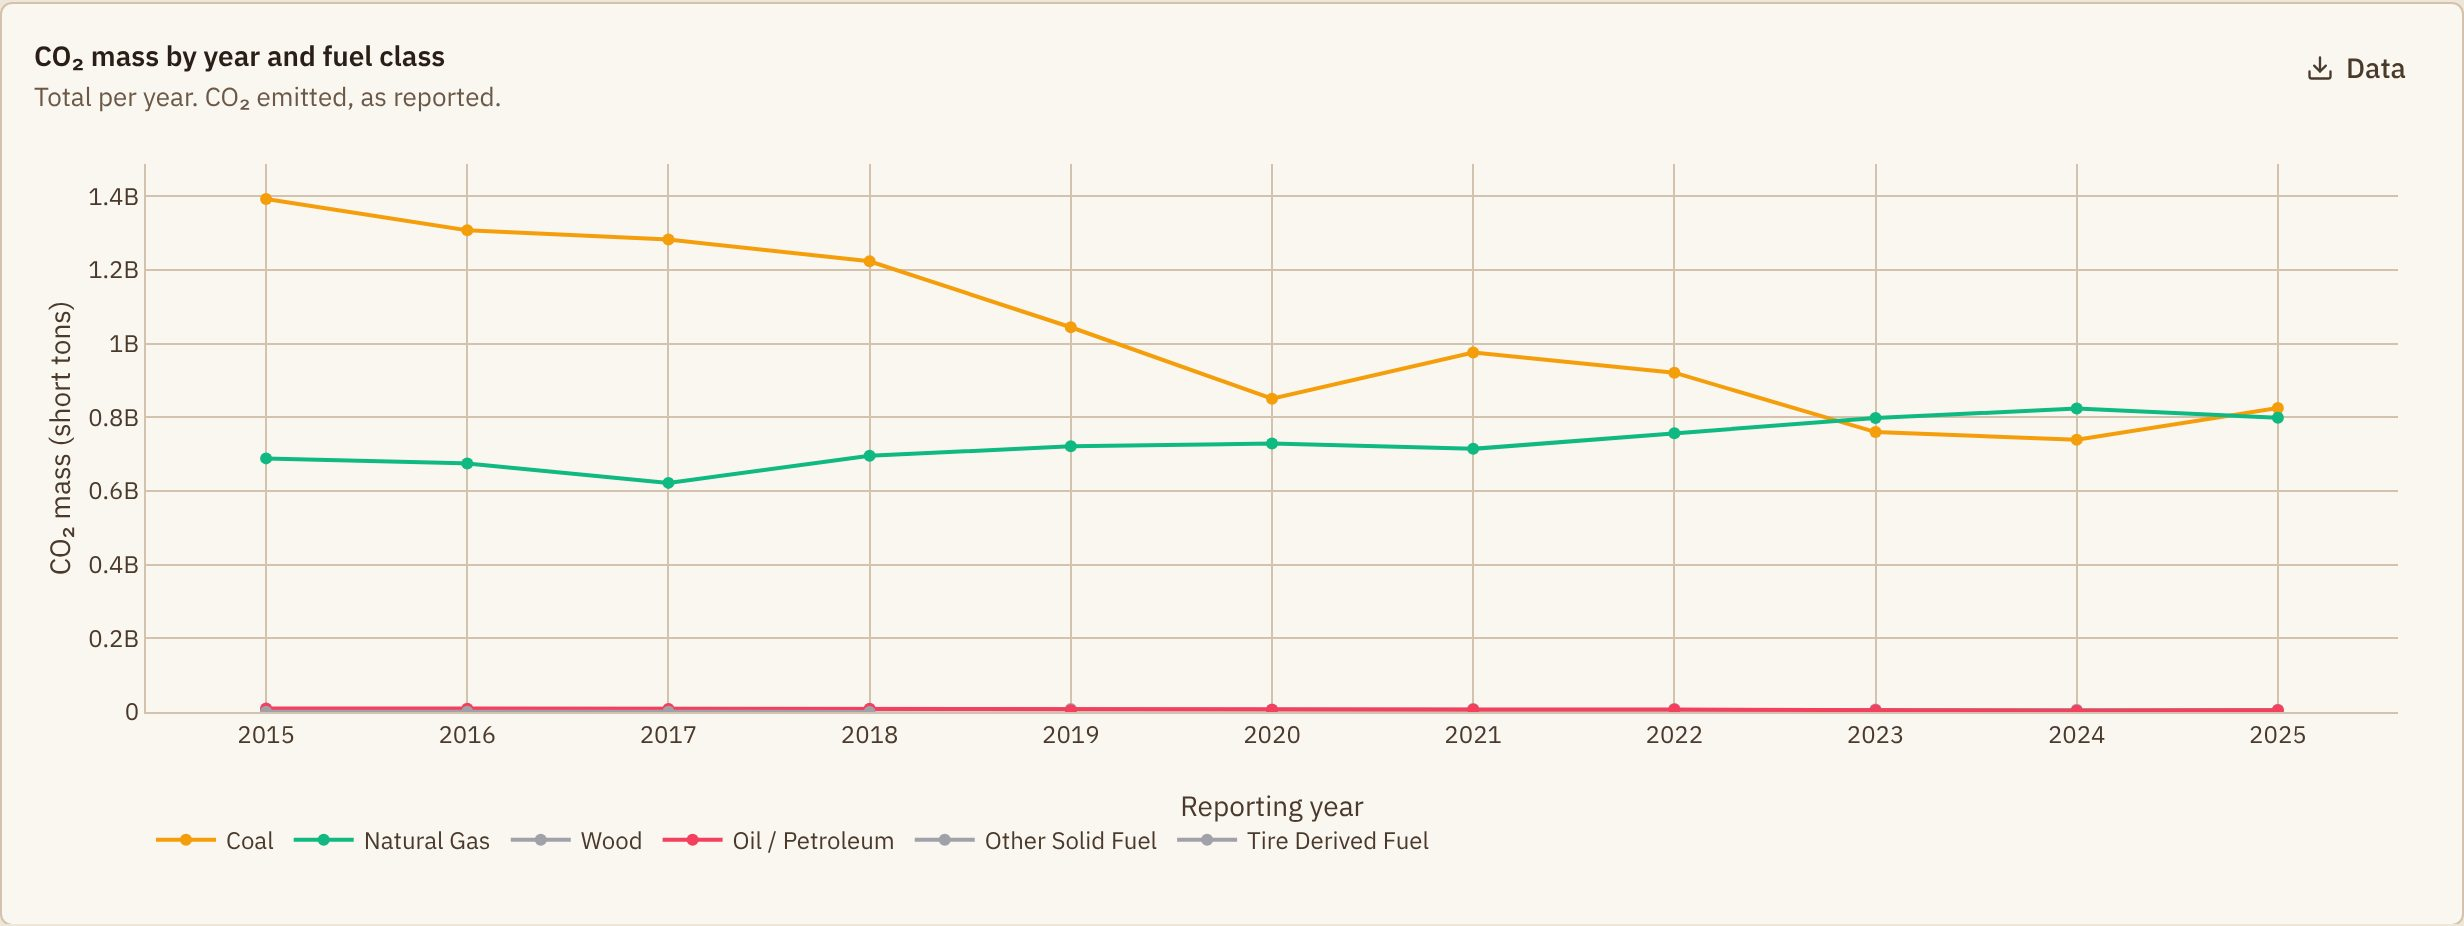
\includegraphics[width=\linewidth]{p2-trend.jpg}
  \caption{Trend chart: total \COtwo{} per year from coal and natural-gas units, 2015--2025.}
  \label{fig:trend}
\end{figure}

\subsection{Q2: \NOx{} rate and post-combustion control}

Figure~\ref{fig:box} shows the \NOx{} emission rate by fuel class on a logarithmic scale. Gas
units have a median of 0.034~lb/MMBtu (interquartile range 0.013--0.096), coal units 0.136
(0.082--0.219), and oil units 0.574 (0.188--1.20), with wide overlap within each fuel.

\begin{figure}[H]
  \centering
  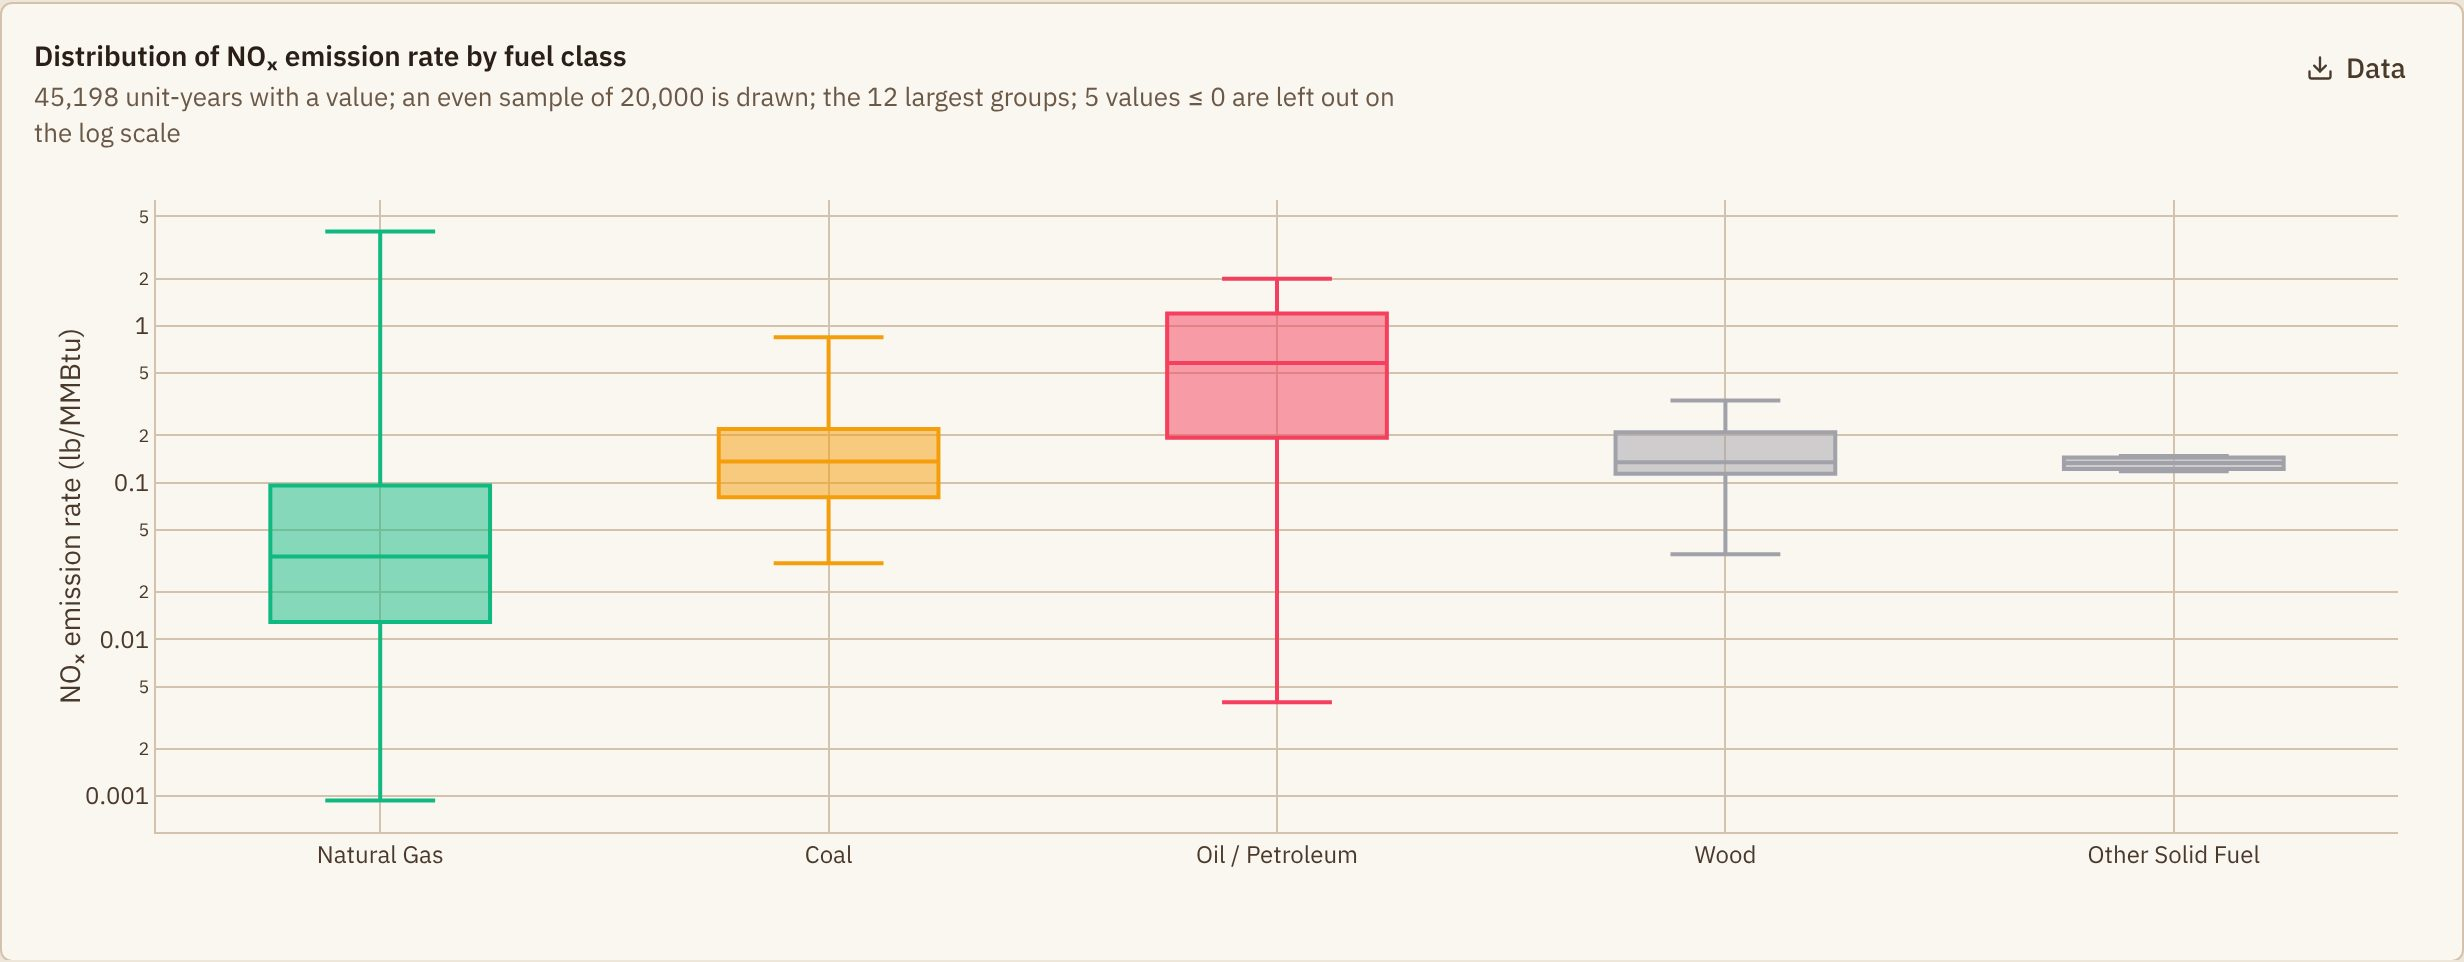
\includegraphics[width=\linewidth]{p2-box.jpg}
  \caption{Box plot of the \NOx{} emission rate by fuel class (log scale).}
  \label{fig:box}
\end{figure}

For 2024, units whose \NOx{} controls include SCR had a pooled rate of 0.037~lb/MMBtu
(1{,}547 unit-years) and units with no reported \NOx{} control 0.159~lb/MMBtu (479 unit-years),
330\,\% higher; the medians were 0.012 and 0.305 (Figure~\ref{fig:compare}). Both Welch's test
($t = -22.3$, $p < 0.001$) and the Mann--Whitney test ($z = -29.8$, $p < 0.001$) reject equal
groups. The difference is real but cannot all be attributed to SCR, because the two groups are
different fleets: 881 of the 1{,}564 SCR unit-years of 2024 are gas combined-cycle units, while
the 571 uncontrolled unit-years are mostly gas combustion turbines and oil units (326 gas and 212
oil). Comparing within one fuel and unit type, which the Compare tab supports by adding those
filters, is the fairer reading.

\begin{figure}[H]
  \centering
  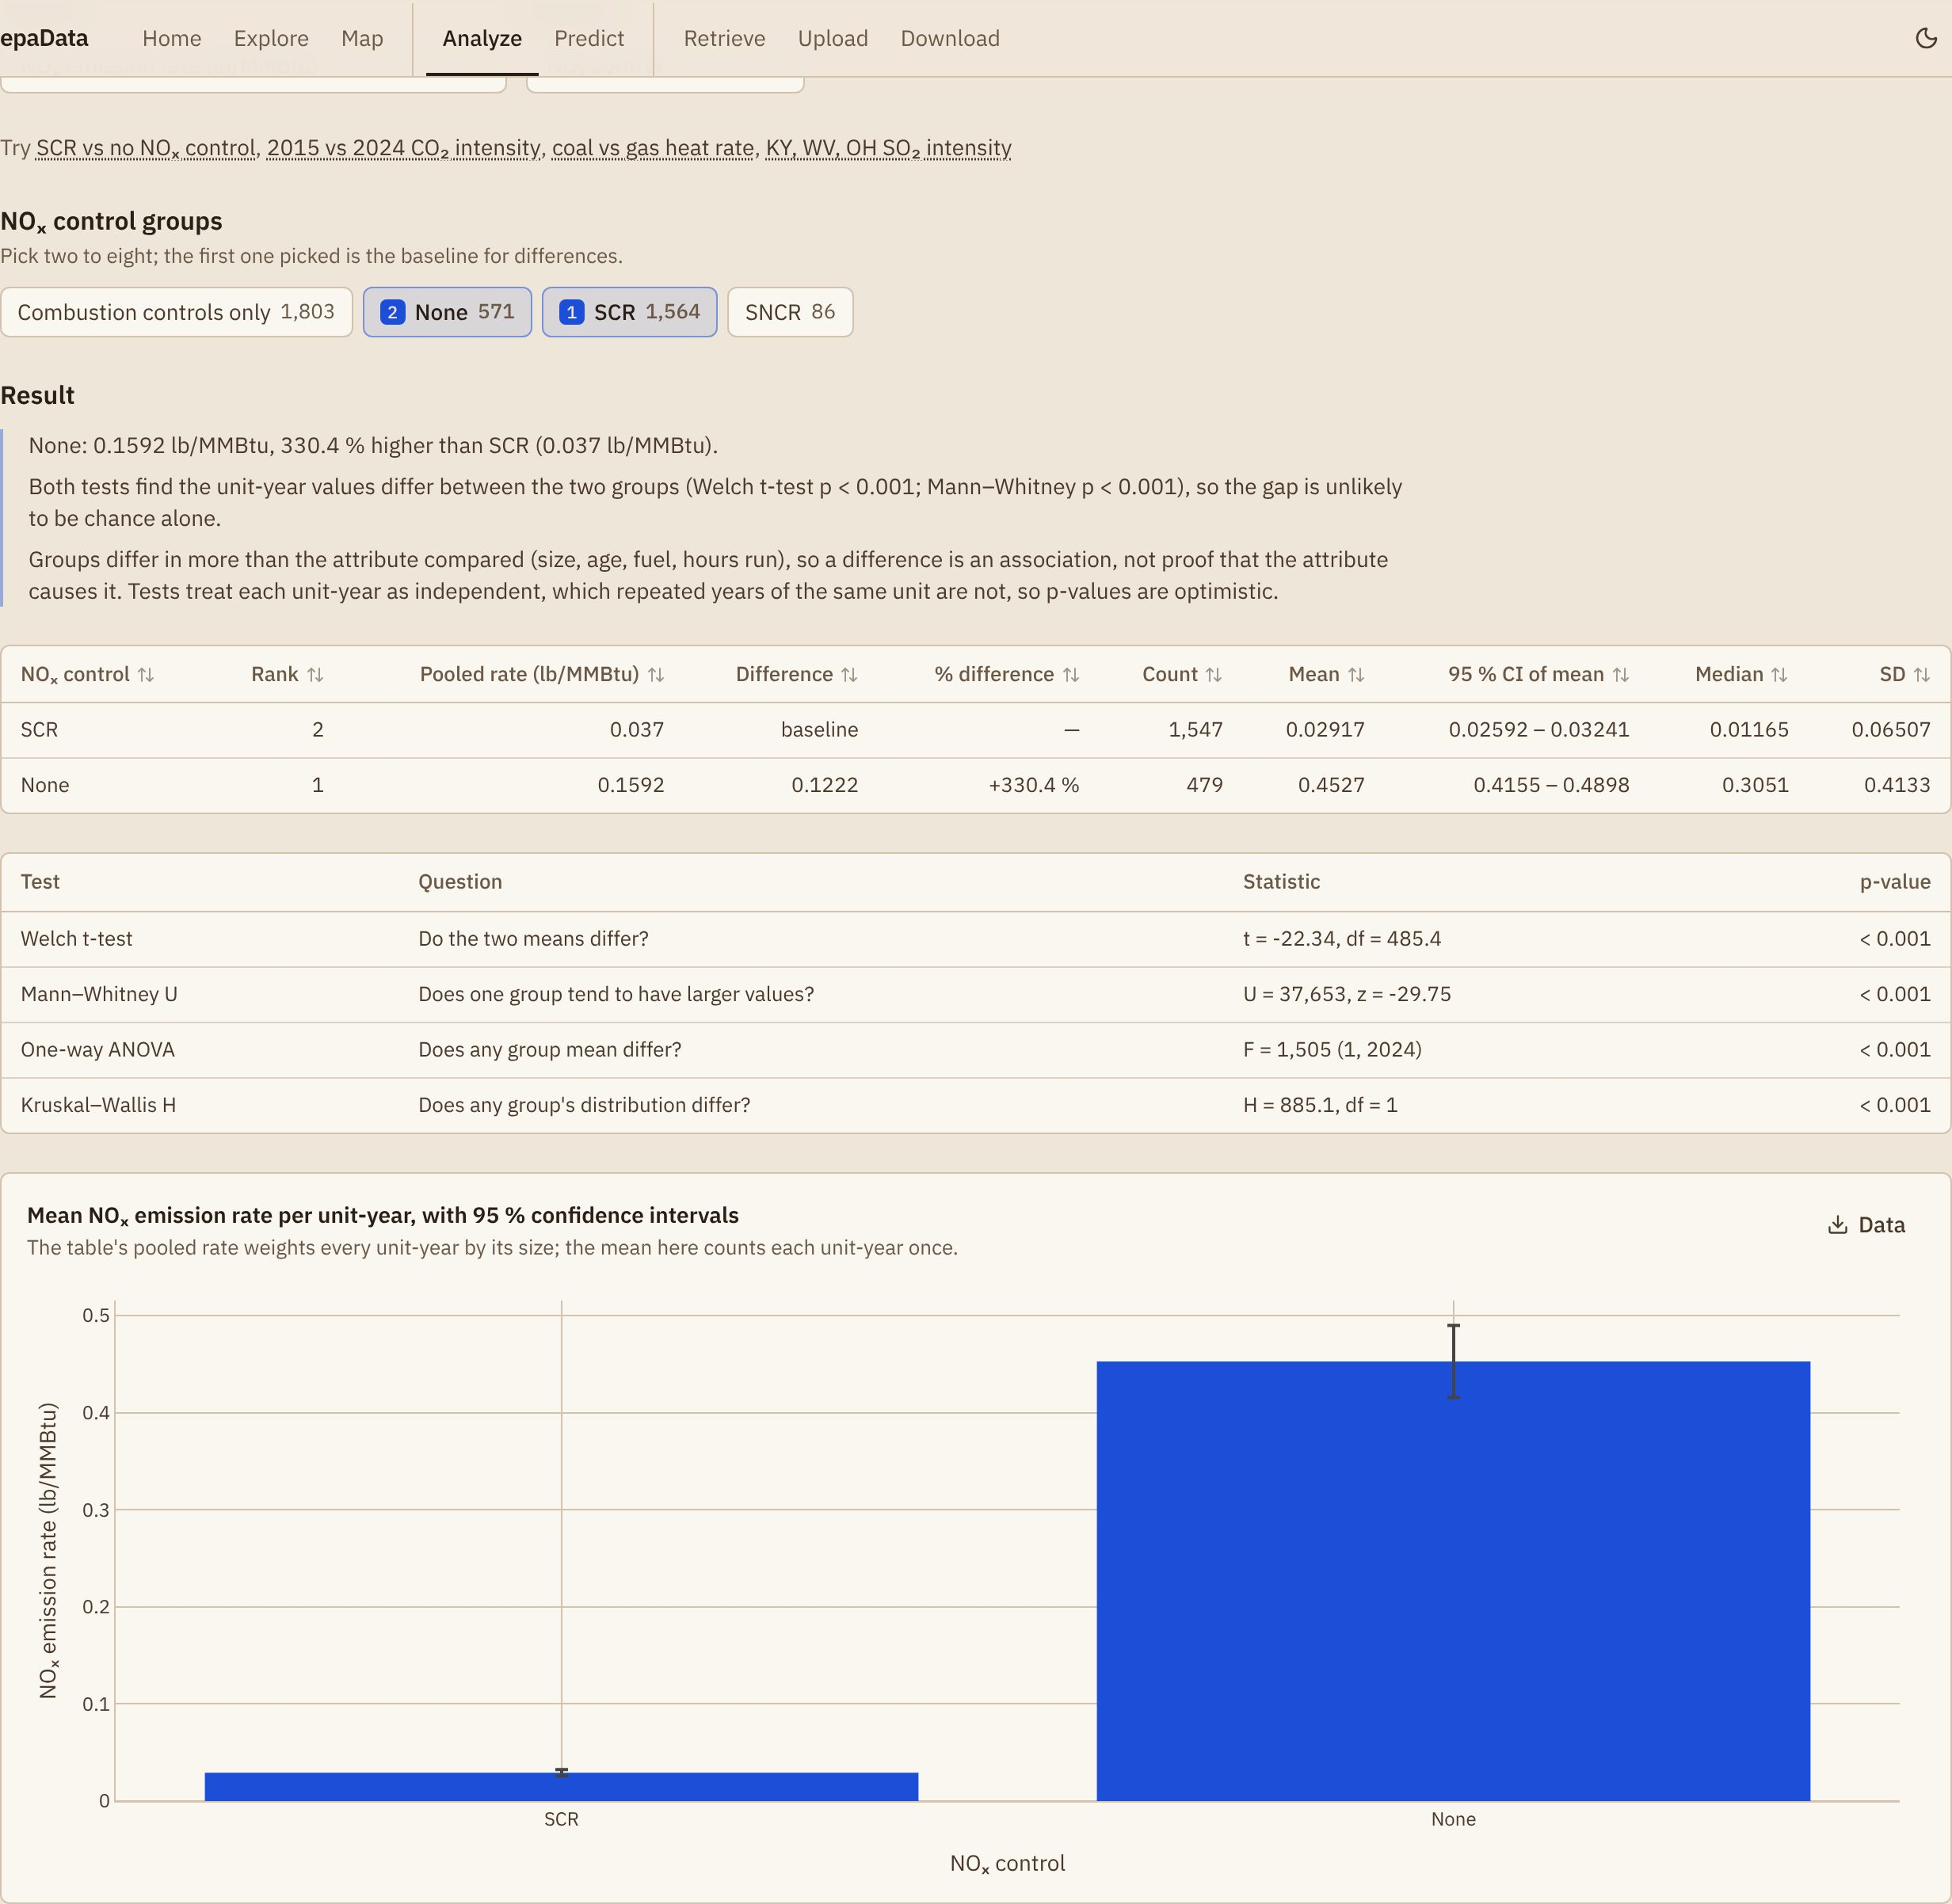
\includegraphics[width=\linewidth]{p2-compare.jpg}
  \caption{Compare tab: \NOx{} emission rate of units with SCR and with no \NOx{} control, 2024.}
  \label{fig:compare}
\end{figure}

\paragraph{Unusual observations.} Over 2015--2025, 3{,}582 unit-years lie above the far-out fence
for \NOx{} intensity (6.1~lb/MWh, against a median of 0.58). Of these, 3{,}491 are combustion
turbines, with a median operating time of 44~hours a year: peaking units whose start-ups produce
\NOx{} with almost no generation. They are real reports rather than errors, but they are why the
pooled rate (0.70~lb/MWh) is the honest summary and the mean (2.46) is not.

\paragraph{A misleading correlation.} The Pearson correlation between \COtwo{} intensity and heat
rate over the 37{,}718 unit-years reporting both is 0.9998, while Spearman's rank correlation is
0.765 (Figure~\ref{fig:correlation}). A few unit-years with tiny gross loads have intensities and
heat rates thousands of times the norm; they dominate Pearson's $r$ and nearly nothing else. The
rank correlation is the honest summary for these heavy-tailed variables, which is why the chart
offers both.

\begin{figure}[H]
  \centering
  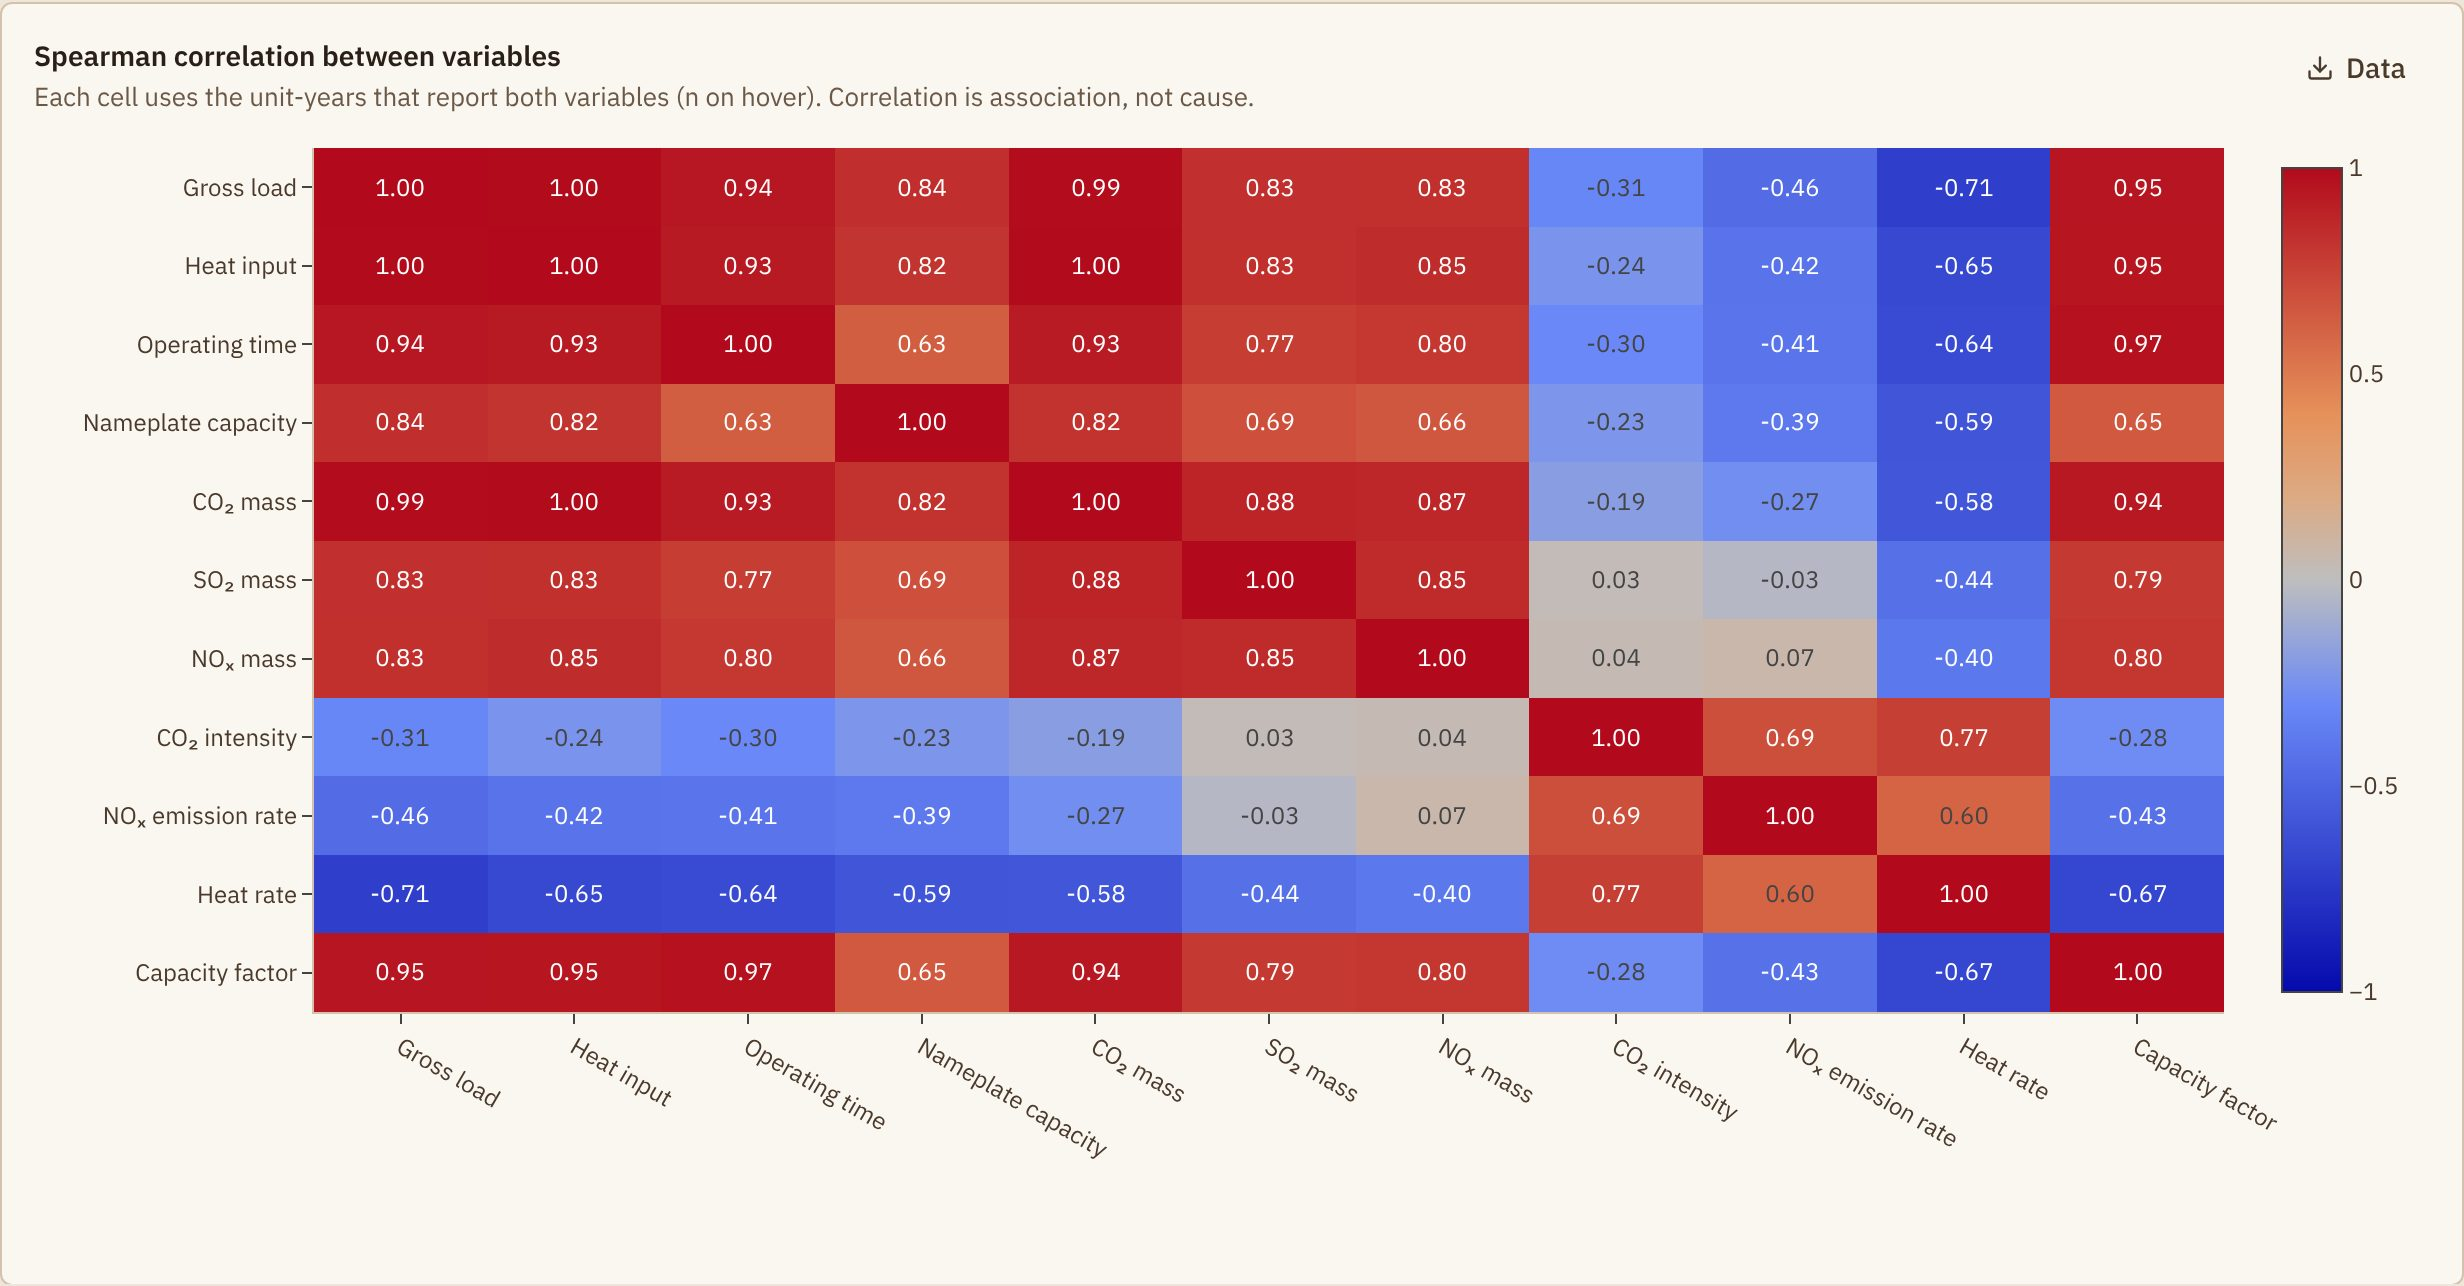
\includegraphics[width=0.85\linewidth]{p2-correlation.jpg}
  \caption{Spearman correlation heat map of eleven variables, 2015--2025.}
  \label{fig:correlation}
\end{figure}

\subsection{Q3: impacts by state}

In 2024 Texas contributed the most to every category: $1.91 \times 10^{11}$~kg \COtwo{}~eq of
global warming and $1.34 \times 10^{8}$~kg \SOtwo{}~eq of acidification, followed for
acidification by Missouri ($7.93 \times 10^{7}$) and Kentucky ($5.65 \times 10^{7}$)
(Figure~\ref{fig:impacts}). Per MWh the ranking changes: Nebraska (2.32~kg \SOtwo{}~eq/MWh),
North Dakota (1.83), and Missouri (1.57) lead. Coal units produced 93\,\% of the reported gross
load of Nebraska and North Dakota and 83\,\% of Missouri's, against 20\,\% in Texas, whose
pooled \SOtwo{} intensity was 0.51~lb/MWh against Nebraska's 3.95. Totals answer where
impacts occur; intensities answer how clean a state's generation is.

\begin{figure}[H]
  \centering
  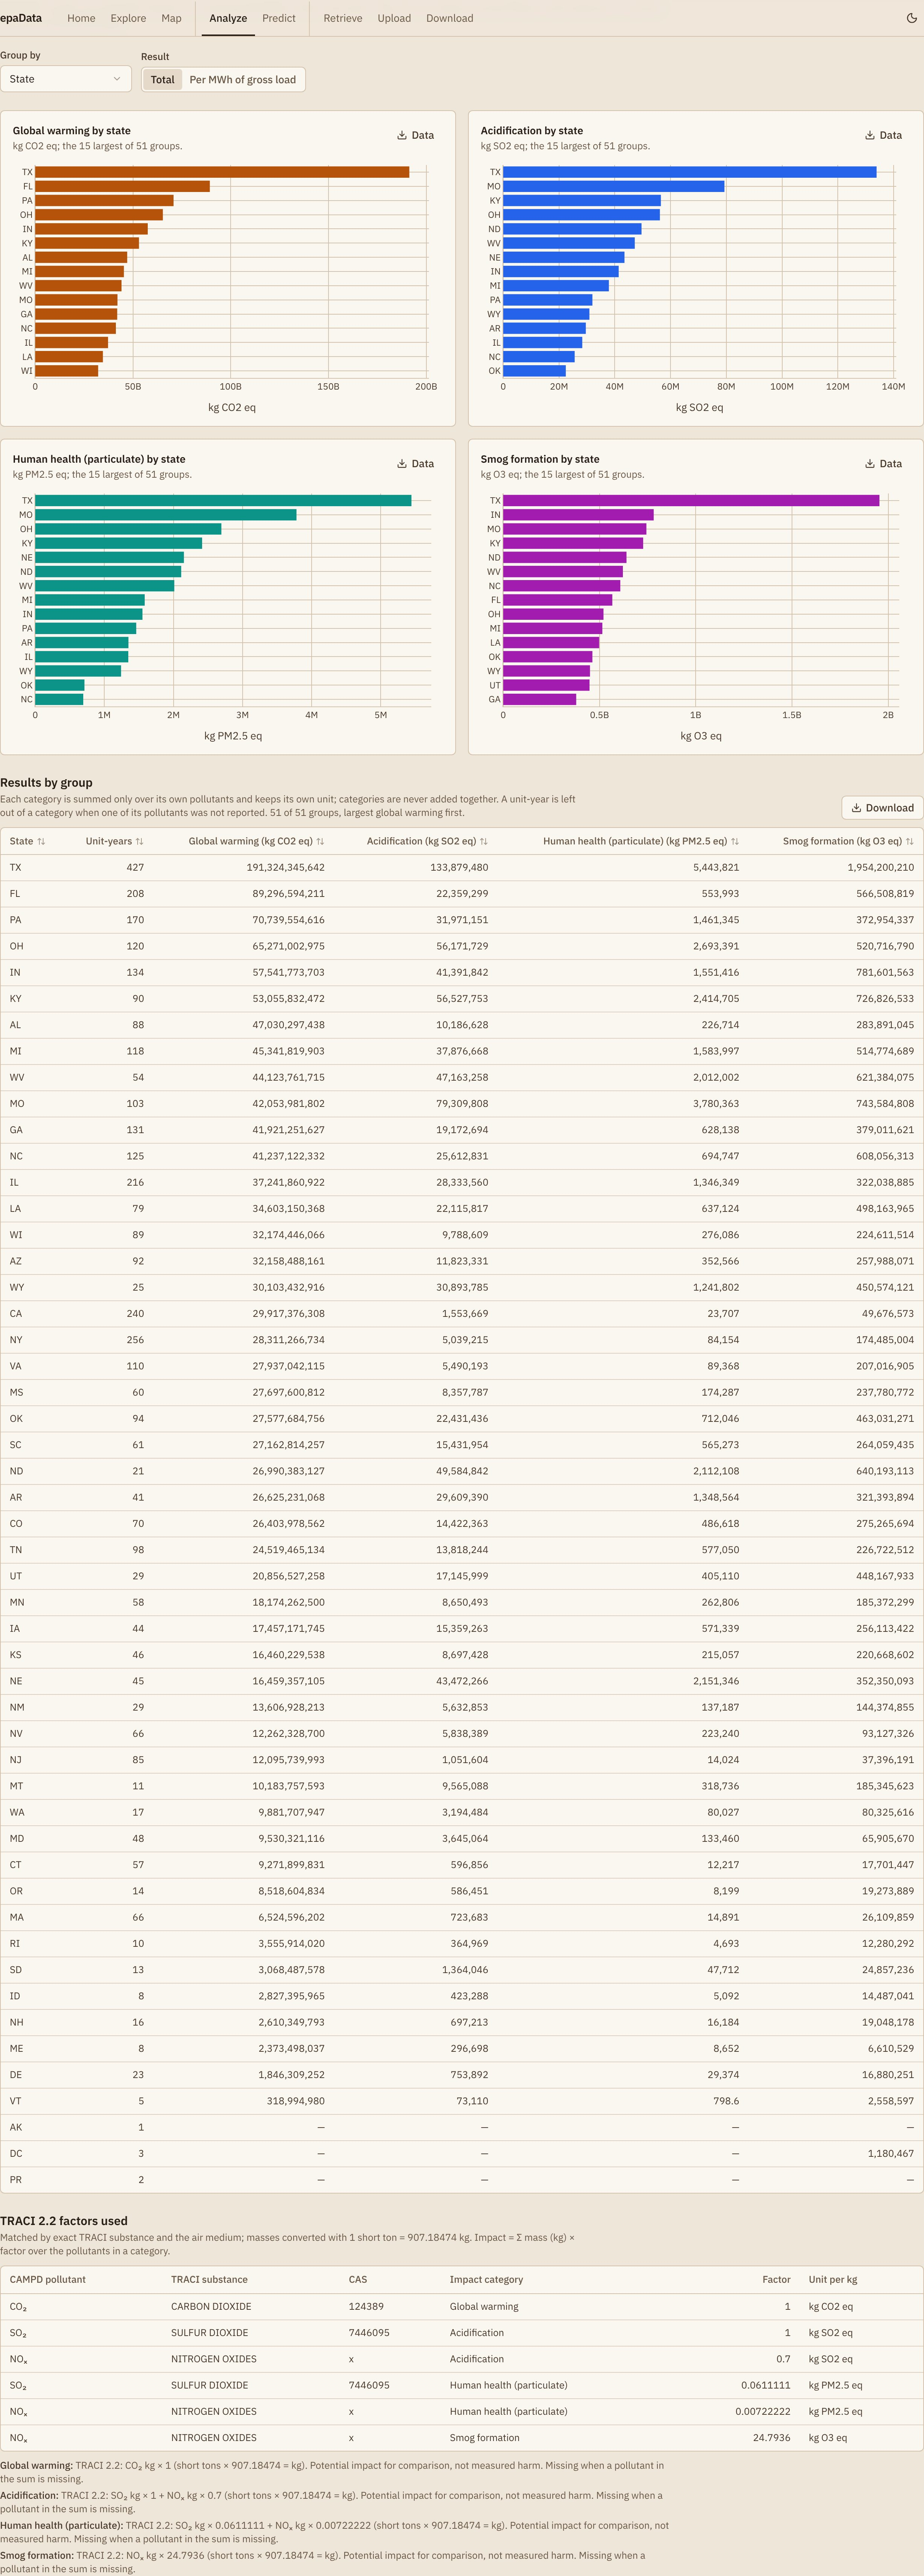
\includegraphics[width=\linewidth]{p2-impacts.jpg}
  \caption{Impacts tab: TRACI categories by state for 2024, each in its own unit.}
  \label{fig:impacts}
\end{figure}

\subsection{Q4: prediction}

Table~\ref{tab:models} compares the models. Both trained models beat the baseline by a wide
margin on the test years: Ridge reduces the MAE by 47\,\% and the tree by 76\,\%. The tree's
validation and test results are close, and so are its training results ($R^2 = 0.956$), so it
does not overfit noticeably despite its depth. Without same-year heat input, gross load, and
operating time, validation $R^2$ falls from 0.853 to 0.704 for Ridge and from 0.967 to 0.837 for
the tree: most of the remaining accuracy comes from the previous year's \NOx{} rate, which
encodes the unit's combustion technology and controls.

\begin{table}[H]
  \centering\small
  \caption{\NOx{} models: validation (2022--2023) and test (2024--2025) results.}\label{tab:models}
  \begin{tabular}{@{}lrrrrrrr@{}}
    \toprule
    & \multicolumn{2}{c}{\textbf{Validation}} & \multicolumn{4}{c}{\textbf{Test}} & \textbf{Ablation}\\
    \cmidrule(lr){2-3}\cmidrule(lr){4-7}\cmidrule(l){8-8}
    \textbf{Model} & MAE (t) & $R^2$ & MAE (t) & RMSE (t) & $R^2$ & MAPE & val.\ $R^2$\\
    \midrule
    Baseline (median by fuel and type) & 114.2 & 0.474 & 109.4 & 366.9 & 0.489 & 143.6\,\% & 0.474\\
    Ridge ($\alpha = 10$, log target) & 57.9 & 0.853 & 58.5 & 213.5 & 0.827 & 49.3\,\% & 0.704\\
    Decision tree (depth 16, leaf 20) & 26.5 & 0.967 & 26.3 & 113.9 & 0.951 & 20.9\,\% & 0.837\\
    \bottomrule
  \end{tabular}
\end{table}

\begin{figure}[H]
  \centering
  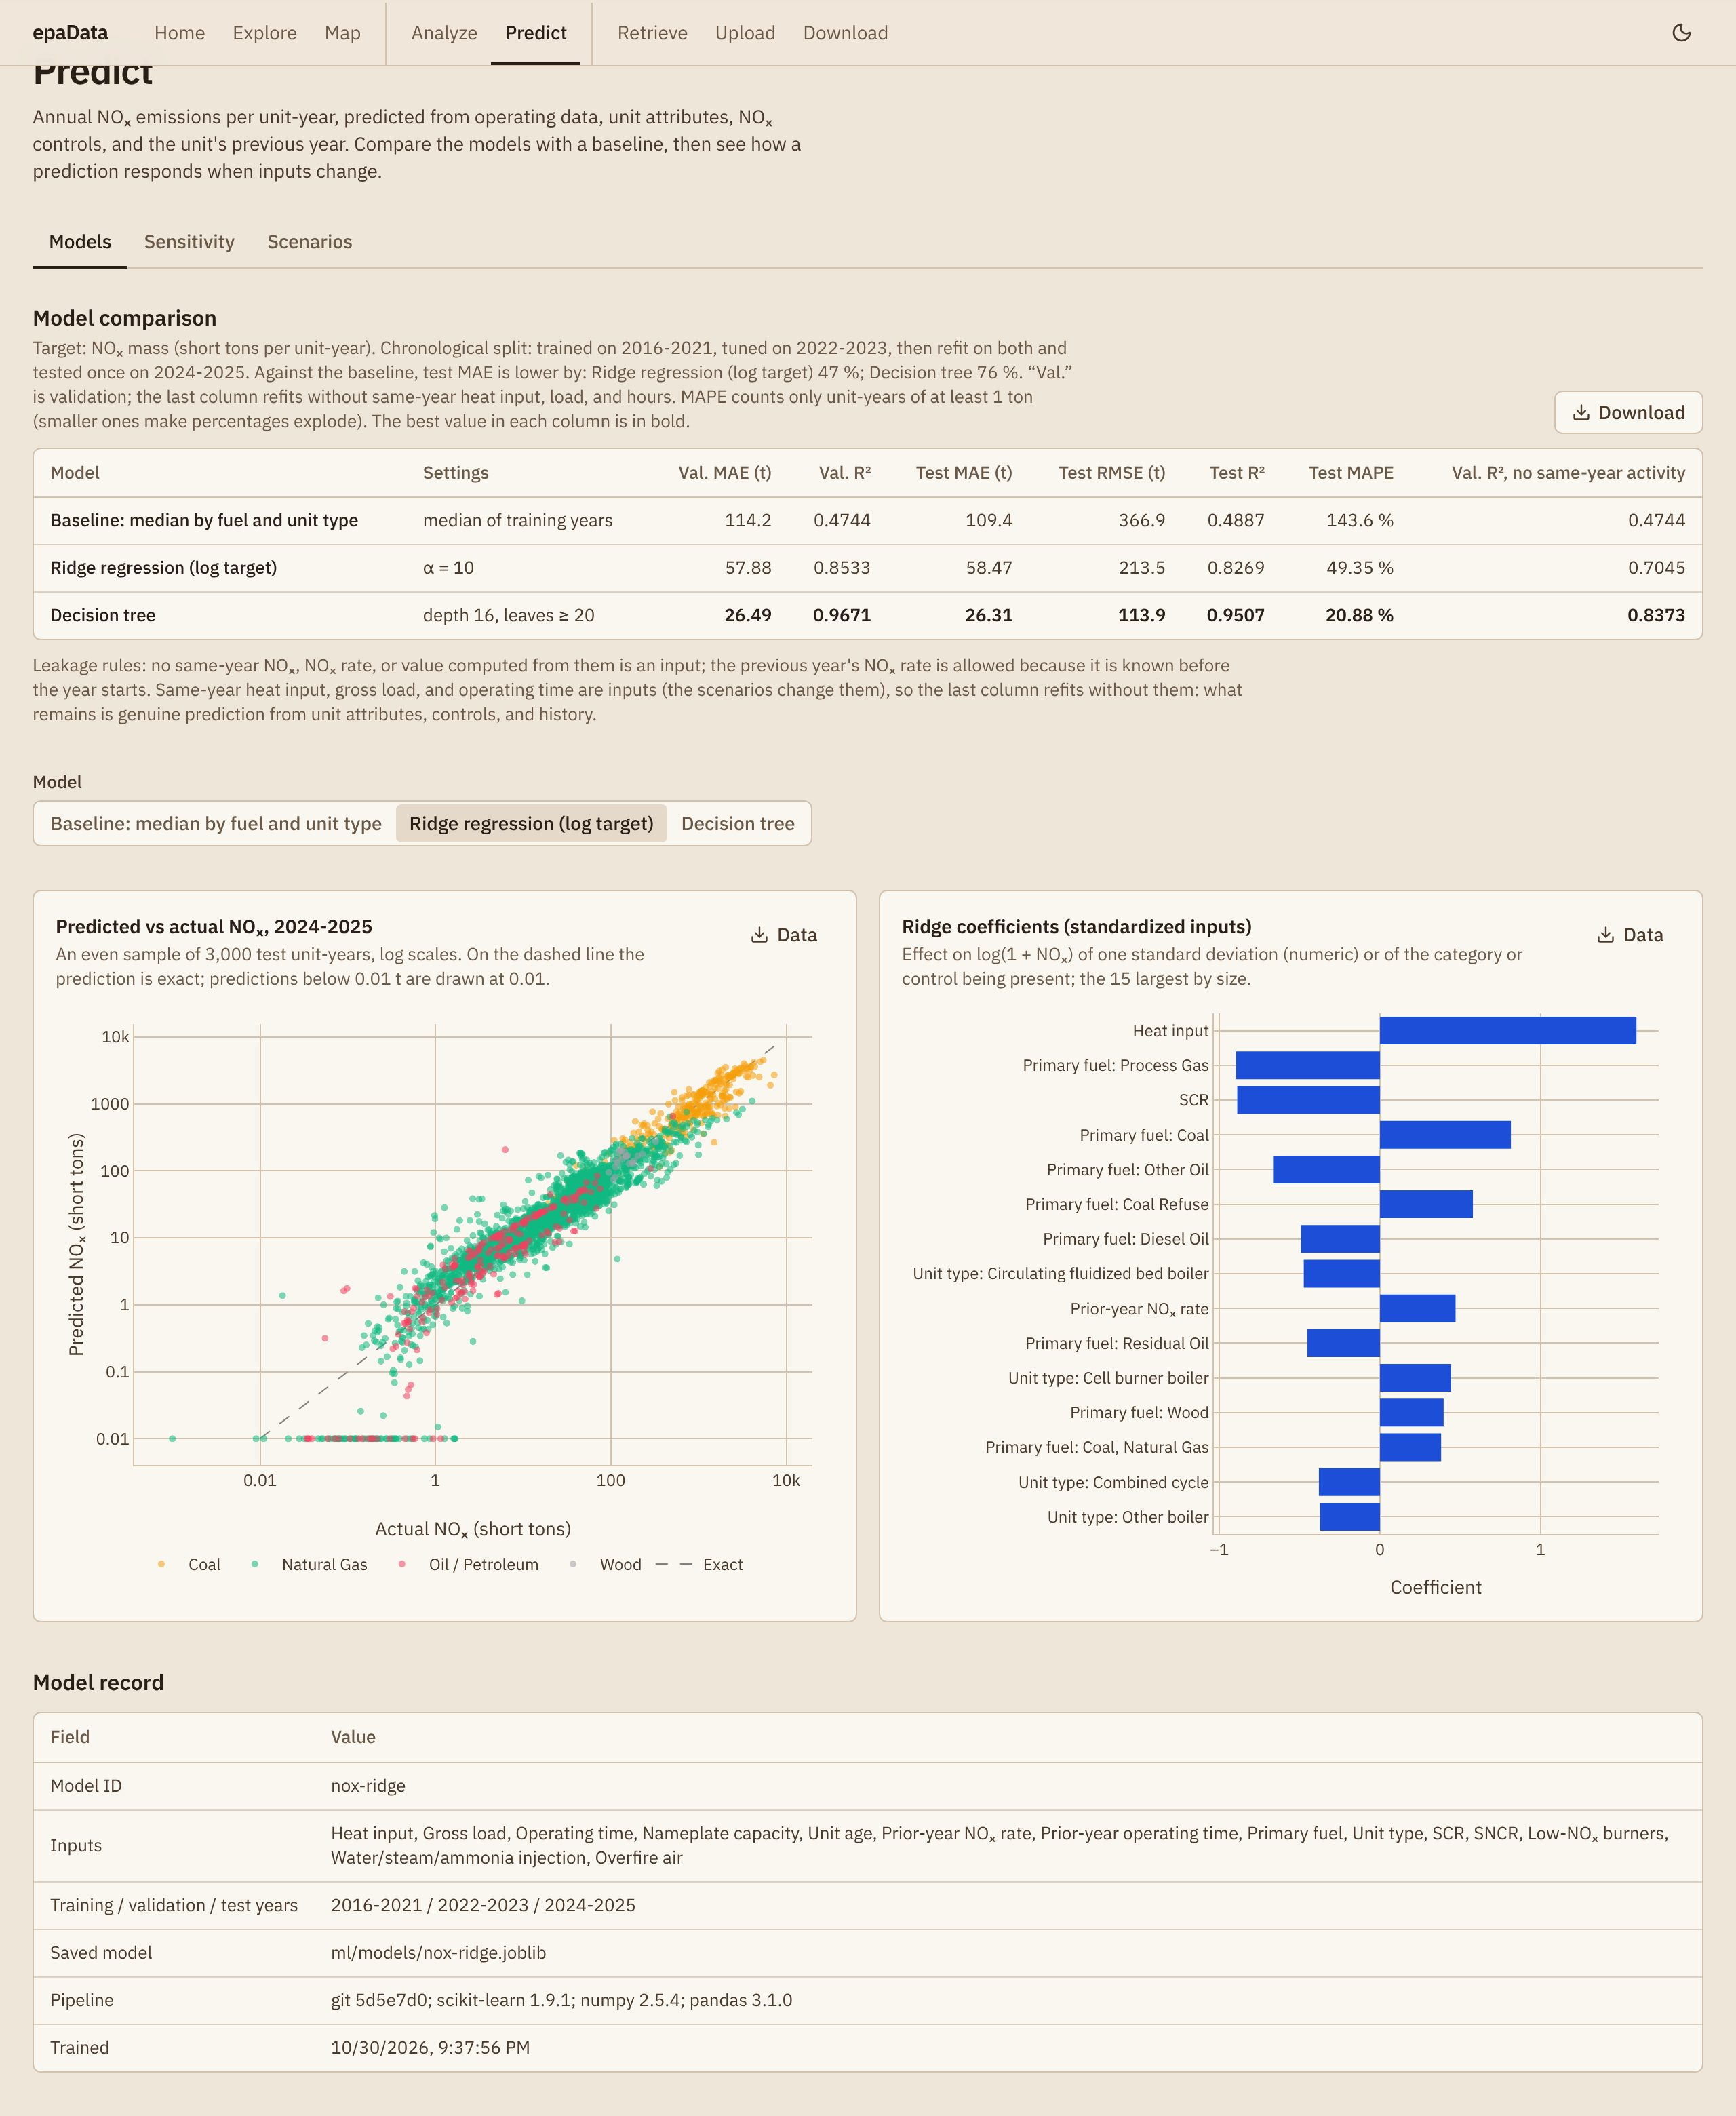
\includegraphics[width=\linewidth]{p2-models.jpg}
  \caption{Models tab: comparison with the baseline, predicted against actual \NOx{} for the
  test years, and the Ridge coefficients.}
  \label{fig:models}
\end{figure}

\paragraph{Sensitivity.} Figure~\ref{fig:sensitivity} varies the heat input of Ghent unit~2 in
2024, a 556~MW tangentially fired coal unit with low-\NOx{} burners and overfire air but no SCR,
which emitted 4{,}146 tons of \NOx{}. Ridge predicts 2{,}972 tons at the baseline; a 50\,\%
increase in heat input raises the prediction to 3{,}827 tons (29\,\%), an elasticity of about
0.6. Beyond 85.8 million MMBtu, the largest heat input in the training years, the curve enters
the shaded region and its points turn amber.

\begin{figure}[H]
  \centering
  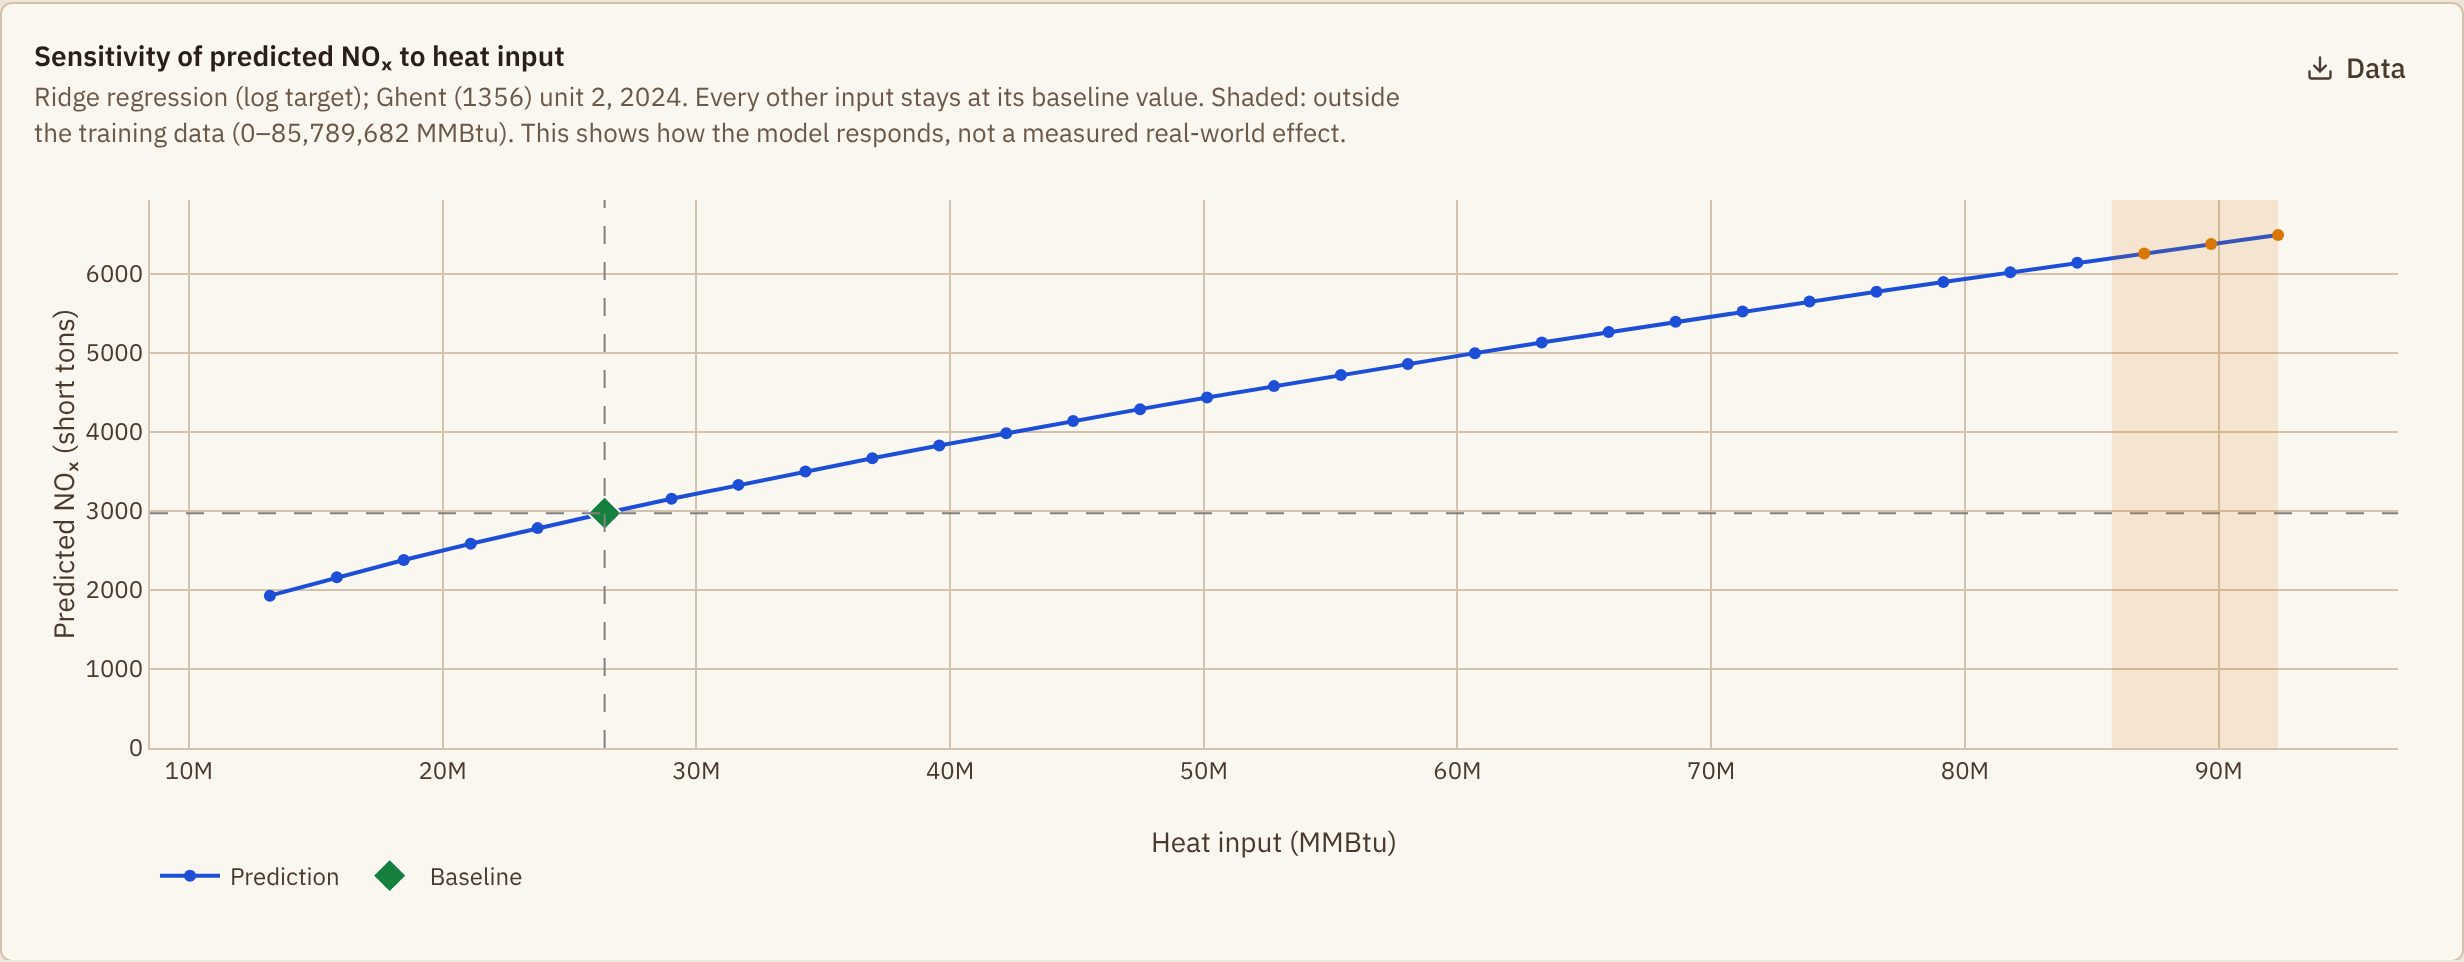
\includegraphics[width=\linewidth]{p2-sensitivity.jpg}
  \caption{Sensitivity of Ridge's \NOx{} prediction to heat input for Ghent unit~2, 2024, from
  $-50\,\%$ to $+250\,\%$. Shaded: outside the training data.}
  \label{fig:sensitivity}
\end{figure}

\paragraph{Scenarios.} Figure~\ref{fig:scenarios} applies the named scenarios to the same unit.
The two models agree on heat input ($-5\,\%$: Ridge $-3.2\,\%$, tree $-9.1\,\%$) and on gross load
(nearly no effect once heat input is fixed), but disagree on controls and fuel. Ridge predicts
that adding SCR would cut \NOx{} by 59\,\% and a switch to pipeline gas by 69\,\%; the tree
predicts no change for either. The tree splits mostly on heat input and the previous year's
\NOx{} rate, which still describes the unit as it was, so a changed control flag rarely changes
its path; Ridge applies one average SCR coefficient to every unit. Neither number is a causal
estimate: where two reasonable models disagree, the data do not settle the effect, and the page
says so.

\begin{figure}[H]
  \centering
  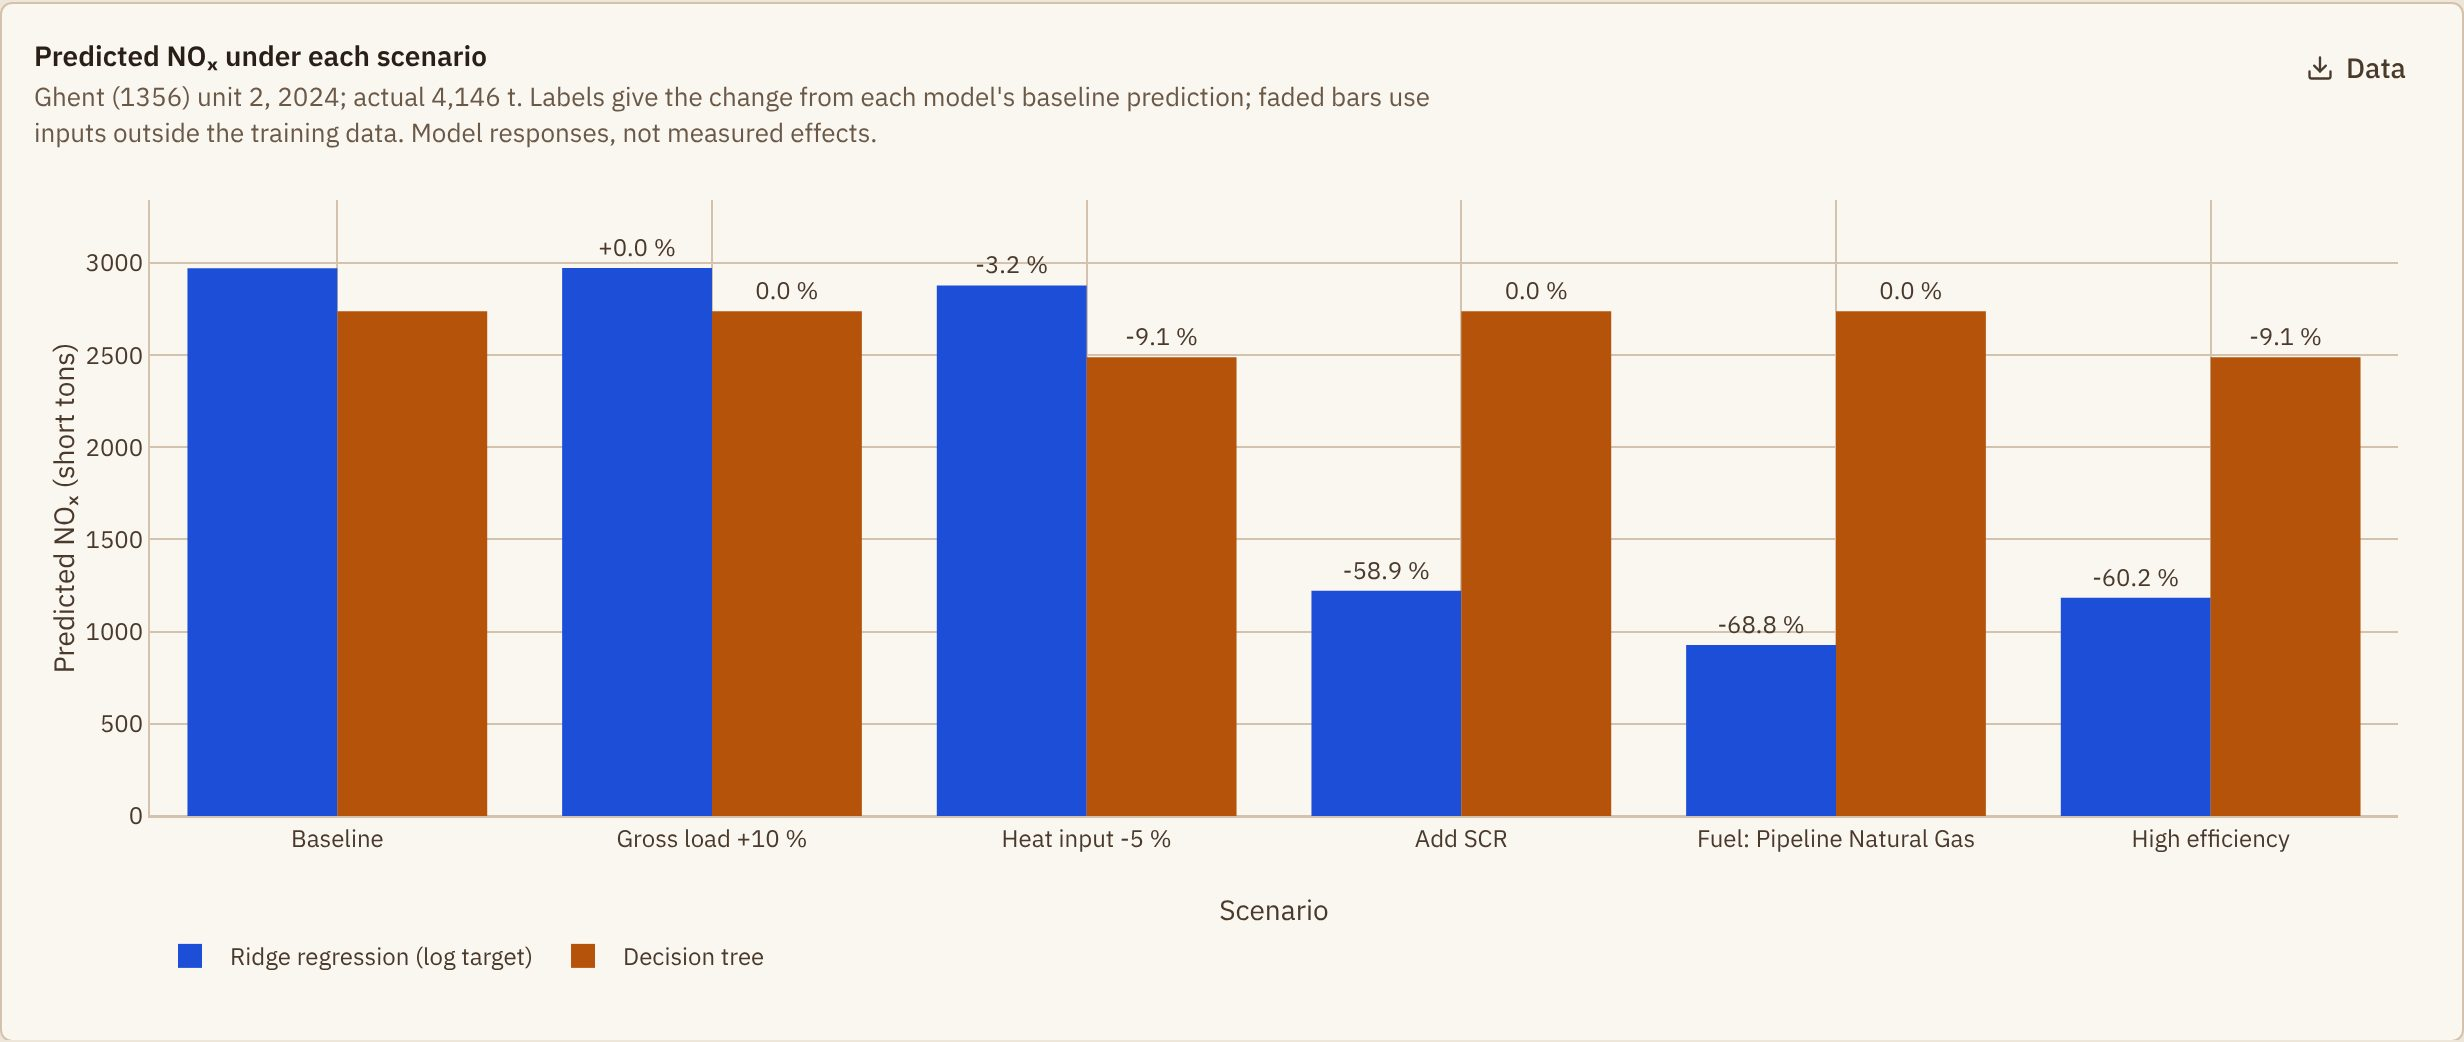
\includegraphics[width=\linewidth]{p2-scenarios.jpg}
  \caption{Scenarios for Ghent unit~2, 2024, under Ridge and the decision tree; labels give the
  change from each model's baseline prediction.}
  \label{fig:scenarios}
\end{figure}

% ------------------------------------------------------------------------
\section{Testing and results}
\label{sec:testing}

\subsection{Approach}

Each calculation was tested against an independent reference: statistics against NumPy and
SciPy, TRACI results against hand calculation, and TypeScript predictions against scikit-learn.
Every page and chart was then exercised in a headless browser (Playwright with Chromium) on the
development and production builds, at desktop and phone widths, checking for console errors and
reading each screenshot; downloaded ZIP files were unpacked and their CSV and metadata checked.
\code{npm run validate} (formatting, linting, type checking, unit tests, and a production build)
passes.

\subsection{Unit tests}

\code{npm test} runs 60 TypeScript tests (one Phase~1 test is skipped), of which these are new:
\begin{itemize}
  \item \code{stats.test.ts}: quantiles and standard deviation against NumPy; Pearson and Spearman
        correlation, Welch's $t$, Mann--Whitney $U$, the confidence interval, ANOVA,
        Kruskal--Wallis, and the $\chi^2$ tail against SciPy, to $10^{-9}$ for statistics and
        $10^{-6}$ for $p$-values; pairwise-complete correlation; constant inputs.
  \item \code{analysis.test.ts}: each derived rate, and its missing value when an input is
        missing or a denominator is zero; capacity factor in leap and ordinary years;
        year-over-year changes with a missing or zero previous year; pooled rates as a ratio of
        sums; TRACI impacts against hand calculation, with categories kept apart and a missing
        pollutant propagating only to its categories; the factor extract (six factors, nitrogen
        oxides rather than nitrogen dioxide); the control classes.
  \item \code{model.test.ts}: the parity test (all three models on 200 test unit-years, within
        $10^{-6}$); input derivation (unit age, control flags, a previous rate that is missing
        when the previous heat input is zero); out-of-range detection; the direction of the
        response to heat input; readable feature names.
  \item The URL state: the default year range applies whenever no filter is in the URL; signed
        percentage formatting.
\end{itemize}
\code{npm run test:py} runs six pytest tests of the training pipeline: the three periods do not
overlap; no input is the target or derived from it; the input rules; the preprocessing
specification produces the same matrix after a round trip through JSON; the baseline is the
group median; and MAPE ignores targets below one ton.

\subsection{Defects found and corrected}

Testing found several defects, all corrected. The 60-second row cache returned a Drizzle query
object rather than its result; Drizzle queries are lazy and re-run on every \code{await}, so the
``cached'' selection was queried again for every view (1.5~s each); the loader now returns a
settled promise and a cached view takes under a millisecond. The server export imported the
module that defined the browser-side export context, which Next.js rejects in server code, so
the dataset export failed; the context moved to the client component that uses it. The
year-range chip, shared with the Explore page, displayed ``2,015--2,025'' (a Phase~1 defect);
years are now shown without separators. A chart's loading placeholder rendered its spinner and
text side by side; the Predict page overflowed a phone screen by ten pixels; both were fixed.
The Python requirements had been pinned to versions that need Python~3.11 or later, while the
documented setup uses Python~3.9; they are now minimum versions that support both.

A final audit against the specification found five more. The emissions-program filter that
\S4.1 lists had never been built, although the filter bar offered controls; it now matches a
whole program code, since CAMPD stores lists such as ``ARP, CSNOX, CSOSG2'' and a substring match
would let ``CSNOX'' catch ``CSNOXOS''. The default 2015--2025 range applied only to a URL with no
parameters at all, so a link to a tab (\code{/analyze?tab=charts}) silently analysed every year
including the partial 2026; it now applies whenever the URL sets no filter. The row cache did not
notice an import for up to a minute; its key now includes the time of the latest import. A
caption wrapped around a segmented control as an HTML \code{label} forwarded a click on the
caption to the first button, flipping the choice; such captions are now plain groups. Finally,
sorting groups whose value was missing used an inconsistent comparison.

\subsection{Assessment against the objectives}

\begin{itemize}
  \item \emph{Descriptive statistics, trends, relationships, unusual observations:} met by the
        Statistics and Charts tabs (Q1, the correlation outlier).
  \item \emph{Comparisons:} met by the Compare tab with tests and plain-language readings (Q2).
  \item \emph{Interactive visualization:} met; seven chart types with export.
  \item \emph{TRACI impacts:} met for the four categories TRACI~2.2 defines for these pollutants
        (Q3).
  \item \emph{Prediction:} met; two models beat the baseline on held-out years (Q4).
  \item \emph{Sensitivity and scenarios:} met, with range warnings.
  \item \emph{Saving and exporting:} met; every result exports with metadata.
  \item \emph{Explaining methods and limitations:} met in the interface (definitions, captions,
        caveats) and in this report.
\end{itemize}

% ------------------------------------------------------------------------
\section{Discussion}
\label{sec:discussion}

\subsection{Effectiveness of techniques and tools}

Treating every derived indicator and TRACI category as an ordinary variable, one definition
with its unit, aggregation rule, and missing-value rule, was the most effective decision of the
phase. Statistics, charts, comparisons, impacts, and exports are each written once and work for
all 29 variables; adding a variable means adding its definition. Reusing the Phase~1 filters
for the analytical dataset meant that the dataset builder came with every filter, its URL
encoding, and its tests already in place.

The offline-training design kept the strengths of both languages: pandas and scikit-learn for
fitting and tuning, and TypeScript for interactive use. Its cost is that preprocessing is
written twice, in \code{train.py} and \code{model.ts}; the parity test is what makes that safe,
and it would catch any change to one that is not made to the other.

\subsection{Technical choices and alternatives}

\paragraph{Flask and pandas at request time.} The specification recommends computing analyses
with pandas behind Flask routes. Rewriting the Phase~1 application in Flask was out of the
question, and calling Python from each request (as Phase~1 does for uploads) would have added
a process start to every chart and would not run on the hosted build. The statistics needed are
few and well defined, so implementing them in TypeScript and checking them against SciPy was
the smaller and safer path.

\paragraph{Plotly.js.} Plotly provides every chart type the specification lists, including box
plots, heat maps, and state maps, together with tooltips, zoom, and PNG export, so a single
component wraps it for all charts. Its bundle is large, so it is loaded only when a chart is
first shown.

\paragraph{Ridge and a decision tree.} The two models were chosen to differ: Ridge is smooth and
gives every input a single global effect, which makes sensitivity curves easy to read; the tree
captures interactions and thresholds, and is far more accurate, but its response to a single
input is a step function and it may ignore an input entirely. The scenario disagreement in
Section~\ref{sec:results} is a direct consequence, and showing both models makes the
uncertainty visible instead of hiding it behind the more accurate one.

\subsection{Challenges and lessons learned}

The TRACI workbook needed care: it lists both nitrogen oxides and nitrogen dioxide with
different smog factors, and it has no eutrophication column, although the plan expected one.
Reading the source rather than relying on a summary avoided both errors. A similar lesson came
from the parity test: a TypeScript reimplementation of a scikit-learn tree that looks correct
still differs in rare cases unless it reproduces the library's 32-bit comparison. Finally, the
correlation outlier showed why statistics over raw emissions data must be robust by default:
a handful of unit-years with almost no generation can produce a near-perfect Pearson correlation
that describes nothing.

% ------------------------------------------------------------------------
\section{Limitations and future improvements}
\label{sec:limitations}

\subsection{Current limitations}

\paragraph{Potential, not actual, impacts.} TRACI factors express potential contributions for
comparison. They do not account for stack height, local population, weather, or background
concentrations, and they say nothing about actual illness or damage. Only the three pollutants
CAMPD reports are covered; particulate matter, mercury, and other emissions are not, and TRACI
2.2 provides no eutrophication factor for these substances.

\paragraph{Missing pollutants remove categories.} A category is missing for a unit-year when one
of its pollutants is not reported. About 13.7\,\% of 2015--2025 unit-years lack \SOtwo{}, so
their acidification and particulate results are missing and group totals cover only the
unit-years that report every contributing pollutant; the Dataset tab shows these counts.

\paragraph{Fuel and unit type are not versioned by year.} As in Phase~1, fuel and unit type are
stored once per unit, so a unit that switched from coal to gas is treated as a gas unit in every
year, both in grouped statistics and as a model input.

\paragraph{Statistical independence.} Unit-years of the same unit are correlated, but the tests
treat them as independent, which overstates their significance. A mixed model or tests on
one value per unit would be more rigorous.

\paragraph{Model responses are not causal.} Both models learn associations in observational data.
A scenario shows how a model responds to a changed input with everything else fixed, which may
be physically impossible (for example more gross load with the same heat input). The previous
year's \NOx{} rate, the most useful history input, also describes the unit's existing controls,
which weakens the models' response to a changed control. Range warnings check each input
separately, not the combination.

\paragraph{Other limitations.} The state map loads the U.S.\ outlines from Plotly's content
network, so it needs internet access. Analysis configurations are saved only as URLs. The
year-over-year variables compare consecutive years only, so a unit with a missing year has no
change for the following year.

\subsection{Future improvements}

Storing fuel and unit type per year, as Phase~1 already proposed, would correct both the grouped
statistics and the model inputs. Tests clustered by unit would give honest $p$-values.
Gradient-boosted trees with monotonic constraints, and models fitted separately for coal and gas,
would likely improve accuracy and make the response to controls more plausible. Joint
out-of-distribution checks (for example a nearest-neighbor distance to the training data) would
make range warnings stricter. Finally, adding the TRACI factors for particulate matter and
mercury would become worthwhile once CAMPD's mercury data are imported.

% ------------------------------------------------------------------------
\section{Individual contributions}
\label{sec:contributions}

The Phase~2 work kept the roles of Phase~1, a back-end and a front-end lead, with testing,
documentation, the report, and the presentation shared.

\paragraph{Raaj Banga (back-end lead).} Responsible for the analytical data layer and the models:
the variable catalogue of derived indicators and year-over-year changes with their
missing-value rules; the statistics and hypothesis tests and their checks against SciPy; the
TRACI~2.2 extract, the \code{traci\_factors} and \code{models} tables, and the impact
calculation; the analysis and prediction procedures and the analytical-dataset export; the
training pipeline in \code{ml/train.py}, the TypeScript inference module, and the parity and
pipeline tests; and the README, \code{DATABASE\_BREAKDOWN.md}, and this report.

\paragraph{Arnav Bawankule (front-end lead).} Responsible for the user interface of Phase~2: the
Analyze page and its Dataset, Statistics, Charts, Compare, and Impacts tabs; the Predict page and
its Models, Sensitivity, and Scenarios tabs; the shared Plotly chart component, its theming,
and the export controls that save each chart and table with its metadata; and the presentation
slides.

% ------------------------------------------------------------------------
\section{References and acknowledgments}
\label{sec:references}

\subsection{Data}

Emissions, operating, facility, and unit data are those of the Phase~1 database, from the EPA
Clean Air Markets Program Data (CAM API, \url{https://www.epa.gov/power-sector/cam-api-portal}),
a U.S.\ government work in the public domain. TRACI~2.2 characterization factors are from the
EPA workbook \code{traci\_2\_2.xlsx}~\cite{epa2022traci22}, downloaded on 30~October 2026
(SHA-256 \code{80383dec\ldots 3725334}); only the six factors in Table~\ref{tab:factors} are
redistributed, in \code{data/traci/}.

\subsection{Reused code and assets}

Phase~2 builds on the Phase~1 code base and its libraries. It adds Plotly.js~\cite{plotly} for
charts, fflate for ZIP files, and, in the offline pipeline, pandas, NumPy, scikit-learn,
joblib, SciPy, and pytest, all used under their open-source licences. No external example code
was copied.

\subsection{Generative AI disclosure}

In accordance with the course policy, we disclose that generative AI was used throughout this
phase. We used Anthropic's Claude, through the Claude Code tool, to help plan the phase, write
and review application, pipeline, and test code, investigate defects, capture screenshots, and
draft the README, the database documentation, and this report. The team defined the analytical
questions, the prediction target, and the design decisions, reviewed all generated code and
text, and accepted changes only after verifying them with the type checker, linter, unit tests,
reference values from NumPy and SciPy, and manual use of the application. Every number in this
report was produced by running the application or the training pipeline against the committed
database. The team takes responsibility for the content of the code and of this report.

\renewcommand{\refname}{Bibliography}
\bibliographystyle{plain}
\bibliography{../shared/refs}

\vfill
\noindent\textit{We used AI to help with this project.}

\end{document}
